\documentclass[11pt]{aghdpl}
% \documentclass[en,11pt]{aghdpl}  % praca w języku angielskim

% Lista wszystkich języków stanowiących języki pozycji bibliograficznych użytych w pracy.
% (Zgodnie z zasadami tworzenia bibliografii każda pozycja powinna zostać utworzona zgodnie z zasadami języka, w którym dana publikacja została napisana.)
\usepackage[english,polish]{babel}

% Użyj polskiego łamania wyrazów (zamiast domyślnego angielskiego).
\usepackage{polski}

\usepackage[utf8]{inputenc}

% dodatkowe pakiety

\usepackage{float}
\usepackage{mathtools}
\usepackage{amsfonts}
\usepackage{amsmath}
\usepackage{amsthm}
\usepackage{siunitx}
%\usepackage{caption}

% \usepackage{tabularx}

% Dodane biblioteki
\usepackage{changepage} % To adjust the width of the column for the title part and figures/tables (adjustwidth environment)
\usepackage{hyperref}

% --- < bibliografia > ---

\usepackage[
style=numeric,
sorting=none,
%
% Zastosuj styl wpisu bibliograficznego właściwy językowi publikacji.
language=autobib,
autolang=other,
% Zapisuj datę dostępu do strony WWW w formacie RRRR-MM-DD.
urldate=edtf,
seconds=true,
% Nie dodawaj numerów stron, na których występuje cytowanie.
backref=false,
% Podawaj ISBN.
isbn=true,
% Nie podawaj URL-i, o ile nie jest to konieczne.
url=false,
%
% Ustawienia związane z polskimi normami dla bibliografii.
maxbibnames=3,
% Jeżeli używamy BibTeXa:
backend=bibtex
]{biblatex}

\usepackage{csquotes}
% Ponieważ `csquotes` nie posiada polskiego stylu, można skorzystać z mocno zbliżonego stylu chorwackiego.
\DeclareQuoteAlias{croatian}{polish}

\addbibresource{bibliografia.bib}

% Nie wyświetlaj wybranych pól.
%\AtEveryBibitem{\clearfield{note}}


% ------------------------
% --- < listingi > ---

% Użyj czcionki kroju Courier.
\usepackage{courier}

\usepackage{listings}
\lstloadlanguages{TeX}

\lstset{
	literate={ą}{{\k{a}}}1
           {ć}{{\'c}}1
           {ę}{{\k{e}}}1
           {ó}{{\'o}}1
           {ń}{{\'n}}1
           {ł}{{\l{}}}1
           {ś}{{\'s}}1
           {ź}{{\'z}}1
           {ż}{{\.z}}1
           {Ą}{{\k{A}}}1
           {Ć}{{\'C}}1
           {Ę}{{\k{E}}}1
           {Ó}{{\'O}}1
           {Ń}{{\'N}}1
           {Ł}{{\L{}}}1
           {Ś}{{\'S}}1
           {Ź}{{\'Z}}1
           {Ż}{{\.Z}}1,
	basicstyle=\footnotesize\ttfamily,
}

% ------------------------

\AtBeginDocument{
	\renewcommand{\tablename}{Tabela}
	\renewcommand{\figurename}{Rys.}
}

% ------------------------
% --- < tabele > ---

\usepackage{array}
\usepackage{tabularx}
\usepackage{multirow}
\usepackage{booktabs}
\usepackage{makecell}
\usepackage[flushleft]{threeparttable}

% defines the X column to use m (\parbox[c]) instead of p (`parbox[t]`)
\newcolumntype{C}[1]{>{\hsize=#1\hsize\centering\arraybackslash}X}


%---------------------------------------------------------------------------

\author{Roman Nowak}
\shortauthor{Roman Nowak}

%\titlePL{Przygotowanie bardzo długiej i pasjonującej pracy dyplomowej w~systemie~\LaTeX}
%\titleEN{Preparation of a very long and fascinating bachelor or master thesis in \LaTeX}

\titlePL{System do detekcji przeszkód zrealizowany z wykorzystaniem kamery zdarzeniowej}
\titleEN{Obstacles detection system using dynamic vision sensor}


\shorttitlePL{Detekcja przeszkód} % skrócona wersja tytułu jeśli jest bardzo długi
\shorttitleEN{DVS obstacles detection}


% Dopuszczalne wartości[1,2]:
% * "Projekt dyplomowy" - na koniec studiów I stopnia
% * "Praca dyplomowa" - na koniec studiów II stopnia
% [1] Zasady dyplomowania w roku akademickim 2020/2021 (Decyzja Dziekana WEAIiIB nr 16/2020 z dnia 9 grudnia 2020 roku)
% [2] Załącznik nr 1a) do Decyzji nr 16/2020 Dziekana Wydziału EAIiIB z dnia 09 grudnia 2020 r.
\thesistype{Projekt dyplomowy}
%\thesistype{Master of Science Thesis}

\supervisor{dr inż. Tomasz Kryjak}
%\supervisor{Paweł Kłeczek, PhD}

\degreeprogramme{Automatyka i Robotyka}
%\degreeprogramme{Automatics and Robotics}

\date{2025}

%\department{Katedra Informatyki Stosowanej}
%\department{Department of Applied Computer Science}

\faculty{Wydział Elektrotechniki, Automatyki, Informatyki i Inżynierii Biomedycznej}
%\faculty{Faculty of Electrical Engineering, Automatics, Computer Science and Biomedical Engineering}

%\acknowledgements{Serdecznie dziękuję \dots tu ciąg dalszych podziękowań np. dla promotora, żony, sąsiada itp.}

\setlength{\cftsecnumwidth}{10mm}

%---------------------------------------------------------------------------
\setcounter{secnumdepth}{4}
\brokenpenalty=10000\relax

% rubber: bibtex.path ./


\newenvironment{abstractpage}
{\cleardoublepage\vspace*{\fill}\thispagestyle{empty}}
{\vfill\cleardoublepage}
\renewenvironment{abstract}[1]
{\bigskip\selectlanguage{#1}%
    \begin{center}\bfseries\abstractname\end{center}}
{\par\bigskip}
\begin{document}

    \titlepages
    % Ponowne zdefiniowanie stylu `plain`, aby usunąć numer strony z pierwszej strony spisu treści i poszczególnych rozdziałów.
    \fancypagestyle{plain}
    {
    	% Usuń nagłówek i stopkę
    	\fancyhf{}
    	% Usuń linie.
    	\renewcommand{\headrulewidth}{0pt}
    	\renewcommand{\footrulewidth}{0pt}
    }

    \begin{abstractpage}
\begin{abstract}{polish}


W ramach niniejszej pracy zrealizowano system detekcji obiektów -- potencjalnych przeszkód dla robota mobilnego (drona) z~wykorzystaniem kamery zdarzeniowej (ang. \textit{Dynamic Vision Sensor (DVS)}). Czujnik ten wykorzystano w~celu zapewnienia poprawnego działania w różnych warunkach oświetleniowych. Przeanalizowano sposoby rozwiązania zagadnienia w~innych projektach dostępnych w literaturze i~na tej podstawie stworzono własny algorytm detekcji. Przygotowano symulację SiL (ang. \textit{Software in the Loop}) umożliwiającą testowanie algorytmu w~świetle dziennym oraz~w nocnych warunkach, oraz tworzenie różnorodnych scen z~przeszkodami. Umieszczono w~niej drona wyposażonego w~symulowaną kamerę zdarzeniową. Przeprowadzono testy systemu wykrywania przeszkód, wykorzystując metodę SiL oraz gotowe zbiory danych z~DVS. Przedstawiono i~omówiono ich wyniki.
% System przetestowano w symulacji SiL (ang. Software-in-the-Loop) oraz na danych rzeczywistych kamer zdarzeniowych. 

%, a następnie przeniesiono na wbudowaną platformę obliczeniową - eGPU Jetson. Dodatkowo, podjęto próbę implementacji systemu na platformie FPGA i uruchomienia na rzeczywistym pojeździe.



\end{abstract}

% \newpage

\begin{abstract}{english}

In this work an object detection system -- obstacles for a~mobile robot (drone) using an event camera (DVS -- Dynamic Vision Sensor) was created. This sensor was applied to ensure correct operation under different lighting conditions. Ways of solving the issue in other designs available in the literature were analysed and a~custom detection algorithm was created. A~SiL (Software in the Loop) simulation was prepared to test the algorithm in daylight and night conditions in variety of scenes with obstacles. A~drone equipped with a simulated event camera was deployed in the scene of testing environment. Tests of the obstacle detection system were carried out using the SiL method and available datasets with DVS data. Their results were presented and discussed.

\end{abstract}
\end{abstractpage}
    \setcounter{tocdepth}{2}
    \tableofcontents
    \clearpage
    
    \chapter{Wprowadzenie}
\label{cha:wprowadzenie}

%---------------------------------------------------------------------------

\section{Cele pracy}
\label{sec:celePracy}


Tu krótko o celach projektu, kolejnych etapach, zamierzonym efekcie końcowym.


%---------------------------------------------------------------------------

\section{Zawartość pracy}

Informacje o zawartości poszczególnych rozdziałów, wykorzystanej bibliografii itd.
\label{sec:zawartoscPracy}

    \chapter{Wstęp teoretyczny}
\label{cha:wstep}

Informacje teoretyczne o wykorzystanych narzędziach, technologiach itp..

%---------------------------------------------------------------------------

\section{Kamery zdarzeniowe}
\label{sec:kamery_zdarzeniowe}

\subsection{Budowa i działanie}

\subsection{Zastosowanie}

\subsection{Rola w projekcie}

\section{Isaac SIM}
\label{sec:isaac_sim}

\subsection{Wprowadzenie}

\subsection{Wykorzystanie w projekcie}

\section{Hardware in the Loop}
\label{sec:hil}

\subsection{Opis metody HIL}

\subsection{Dlaczego ten sposób testowania?}

\section{Układy FPGA}
\label{sec:fpga}

\subsection{Budowa i działanie - podstawy}

\subsection{Przewaga nad wykorzystaniem CPU w kontekście projektu}




    \chapter{Przegląd literatury}
\label{cha:literatura}

Problem skutecznej detekcji oraz unikania przeszkód przez roboty mobilne lub drony często pojawia się w projektach z dziedziny robotyki opisanych w literaturze. Potrzeba integracji takich systemów wynika z chęci zwiększenia ich autonomiczności -- każdy system sterowania robotem mobilnym, który ma działać samodzielnie, bez ingerencji operatora, musi być wyposażony w system pełniący taką funkcję.

Do detekcji zagrożeń na trasie robota często wykorzystuje się proste czujniki zbliżeniowe lub czujniki odległości. W ten sposób jednak uzyskuje się jedynie stosunkowo późną informację o obecności lub dodatkowo o odległości do przeszkody. Takie podejście okaże się wystarczające, jeśli robot porusza się wolno, przeszkody są duże i nieruchome, a wymagana reakcja robota na wystąpienie barier na trasie nie wymaga żadnych dodatkowych danych (przykładowo -- robot skręca w prawo o 90 stopni, za każdym razem gdy napotka przeszkodę).

Realizowany w ramach projektu system powinien jednak mieć szersze możliwości. Oprócz dostarczania danych o wystąpieniu przeszkody, ma on za zadanie informować także o jej położeniu, kształcie oraz prędkości, a wszystko to odpowiednio wcześnie, tak aby możliwe było zaplanowanie trajektorii i zapewniona możliwość szybkiego przemieszczania się robota. Takie podejście do problemu daje możliwości reakcji na przeszkody będące w ruchu oraz na realizację bardziej złożonych algorytmów sterowania w celu ich skutecznego uniknięcia.

% Ta część może pójdzie do terii potem
Sposoby wykrywania przeszkód zebrane i~opisane są w~artykułach \cite{detection_techniques}, \cite{detection_methods} oraz w~\cite{detection_methods2}. Detekcja obiektów może być realizowana na podstawie danych pochodzących z~różnych typów czujników. Najczęściej wykorzystywane sensory to:
\begin{itemize}
    \item LiDAR (ang. \textit{Light Detection and Ranging}) -- czujnik zbierający przestrzenne dane o~otoczeniu (odległości do otaczających go obiektów), za pomocą krótkich sygnałów świetlnych. Główną zaletą jest wysoka precyzja, natomiast wadą -- duża ilość danych, które należy przetworzyć, a~więc wysokie wymagania obliczeniowe systemów opartych na tych czujnikach.
    \item RADAR (ang. \textit{Radio Detection and Ranging}) -- działa dzięki sygnałom radiowym. Charakteryzuje się potencjalnie dużym dystansem detekcji, ale może mieć problem z~wykrywaniem obiektów niewielkich oraz takich, które słabo odbijają fale w~tym zakresie.
    \item SONAR (ang. \textit{Sound Navigation and Ranging}) -- wykorzystuje sygnały dźwiękowe i~używany jest głównie tam, gdzie warunki negatywnie wpływają na działanie innych czujników (np. pod wodą).
    \item Czujniki ultradźwiękowe -- to urządzenia wykorzystujące fale dźwiękowe o~wysokiej częstotliwości (powyżej zakresu słyszalnego dla ludzkiego ucha, tj. > \SI{20}{kHz}) do wykrywania obiektów i~mierzenia odległości. Działają na zasadzie emisji ultradźwięków i~analizy echa odbitego od przeszkody. Ich zaletą jest niezależność od oświetlenia sceny i~niski koszt, natomiast wadą stosunkowo niewielki dystans detekcji.
    \item Kamery -- niewątpliwą zaletą ich stosowania jest niska cena. % w porównaniu do czujników aktywnych (czyli posiadających własne źródło energii -- wszystkie powyższe).
    Wykorzystując kamery do detekcji obiektów, stosuje się różne podejścia. Przeszkody można wykrywać na podstawie ich znanych właściwości -- kształtu i~rozmiaru, lub na podstawie ich ruchu i~prędkości. Projektuje się systemy wykorzystujące pojedynczą kamerę, jak i~takie z dwiema kamerami skonfigurowanymi w~układ stereo, co daje większe możliwości przy obliczaniu głębi.
   %\item Czujniki ultradźwiękowe to urządzenia wykorzystujące fale dźwiękowe o~wysokiej częstotliwości (powyżej zakresu słyszalnego dla ludzkiego ucha, tj. >\SI{20}{kHz}) do wykrywania obiektów i~mierzenia odległości. Działają na zasadzie emisji ultradźwięków i~analizy echa odbitego od przeszkody. Ich zaletą jest niezależność od oświetlenia sceny i~niski koszt, natomiast wadą stosunkow niewielki dystans detekcji.
    \item \textbf{Kamery zdarzeniowe} -- szerzej opisane w~podrozdziale \ref{sec:kamery_zdarzeniowe}
\end{itemize}

% \section{Powiązane publikacje}
% \label{sec:przeglad}

W~literaturze znaleźć można artykuły opisujące projekty o~podobnej tematyce, w~ramach których został zaprojektowany i~zaimplementowany system detekcji i~unikania przeszkód. W~celu wyboru metody rozwiązania tego problemu przeanalizowano sposoby detekcji zastosowane w~wybranych, najbardziej zbliżonych do tematu projektu publikacjach. Cele w~tych artykułach częściowo pokrywają się z~celami projektu (\ref{sec:celePracy}), co pozwala na wzorowanie się na nich i~czyni je szczególnie pomocnymi~w realizacji zadania. 

\textbf{Dynamic obstacle avoidance for quadrotors with event cameras} (\textit{Davide Falanga, Kevin Kleber, Davide Scaramuzza}) \cite{dynamic_obstacle} -- projekt, w~którym autorzy zaprojektowali i~zaimplementowali system unikania przeszkód dla czterowirnikowego drona. Celem było ominięcie szybko poruszających się (do \SI{10}{\frac{m}{s}}) w~kierunku drona obiektów (na przykład rzuconej w~niego piłki -- rys. \ref{fig:dynamic_obstacle}). Statyczne bariery na trasie drona są ignorowane. System działa zarówno na zewnątrz, jak i~we wnętrzach budynków. Autorzy, oprócz skuteczności, skupiają się na osiągnięciu możliwie niskiej latencji w~wykrywaniu przeszkód -- końcowa wartość to $3.5$ $ms$. Jest to możliwe właśnie dzięki zastosowaniu kamer zdarzeniowych.

\begin{figure}
    \centering
    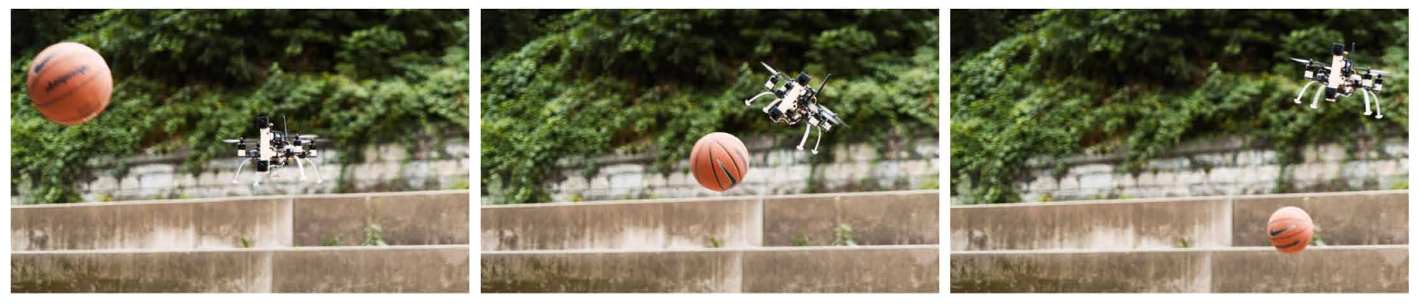
\includegraphics[width=0.8\linewidth]{images/dyanimc_obstacle.png}
    \caption{Przykład manewru uniku z projektu \cite{dynamic_obstacle}.}
    \label{fig:dynamic_obstacle}
\end{figure}

Na system detekcji przeszkód z~projektu \cite{dynamic_obstacle} składają się kolejne etapy:
\begin{enumerate}
    \item Kompensacja ruchu własnego drona -- autorom zależy na wykrywaniu wyłącznie poruszających się przeszkód, jednak zdarzenia w DVS generowane są również przez ruch  samego drona i~obiekty statyczne. Na podstawie danych z czujnika IMU (ang. \textit{inertial measurement unit}) -- rotacji drona, odróżniane są statyczne elementy sceny od dynamicznych.
    \item Segmentacja przeszkód -- dzięki wynikom poprzedniego etapu możliwe jest oddzielenie zdarzeń odpowiadających za przeszkody od statycznej części sceny. Dalej przetwarzane są tylko obiekty w~ruchu.
    \item Obliczenie przepływu optycznego za pomocą algorytmu Lucasa-Kanade \cite{Lucas-Kanade}, w~celu usprawnienia późniejszej klasteryzacji zdarzeń. Przepływ optyczny dostarcza dane o wektorach ruchu pikseli na obrazie, co ułatwia odróżnienie różnych obiektów, które znajdują się blisko siebie, ale poruszają się inaczej.
    \item Klasteryzacja -- za pomocą algorytmu DBScan \cite{DBScan} separuje się zdarzenia odpowiadające poszczególnym obiektom -- scena może zawierać wiele przeszkód. Dodatkową rolą tego etapu jest usunięcie szumu.
    \item Estymacja pozycji w przestrzeni 3D -- w~przypadku gdy używana jest tylko jedna kamera zdarzeniowa, autorzy w celu wyznaczenia głębi, ograniczają się do przeszkód o~znanym rozmiarze. Wtedy ich odległość od kamery może być łatwo wyznaczona na podstawie ich szerokości w~klatce obrazu.
    W~przypadku dwóch kamer w układzie stereo \cite{detection_methods}, możliwa jest estymacja głębi dla wszystkich obiektów za pomocą triangulacji \cite{view_geometry}.
    \item Projekcja pozycji przeszkód z układu współrzędnych kamery na układ współrzędnych świata i~estymacja prędkości przeszkód.

\end{enumerate}

\textbf{EVDodgeNet: Deep Dynamic Obstacle Dodging with Event Cameras} (\textit{Nitin J. Sanket, Chethan M. Parameshwara, Chahat Deep Singh, Ashwin V. Kuruttukulam,
Cornelia Fermüller, Davide Scaramuzza, Yiannis Aloimonos}) \cite{EVDodge} -- projekt, w którym problem zdefiniowany jest bardzo podobnie do \cite{dynamic_obstacle} -- unikanie przez drona szybko poruszających się obiektów różnych kształtów i~rozmiarów. Podejście do implementacji znacznie się jednak różni. Autorzy do kolejnych etapów detekcji obiektów na podstawie danych z~kamery zdarzeniowej wykorzystują szereg płytkich sieci neuronowych. Pierwsza z~nich odpowiedzialna jest za poprawę jakości ramek zdarzeniowych (usunięcie rozmycia, redukcja szumów). Kolejna odpowiada za uzyskiwanie odometrii (estymacja pozycji). Zadaniem ostatniej jest segmentacja niezależnie poruszających się obiektów. Modele trenowane były wyłącznie przy wykorzystaniu symulacji komputerowej. Skuteczność gotowego systemu autorzy oceniają na $70\%$. System przetestowany został również w~trudnych warunkach oświetleniowych, w~których mógł efektywnie pracować, dzięki zastosowaniu DVS. 

\textbf{Night vision obstacle detection and avoidance based on Bio-Inspired Vision Sensors} (\textit{Jawad Naveed Yasin,
                  Sherif Abdelmonem Sayed Mohamed,
                  Mohammad Hashem Haghbayan,
                  Jukka Heikkonen,
                  Hannu Tenhunen,
                  Muhammad Mehboob Yasin,
                  Juha Plosila}) \cite{night_obstacle} -
    projekt, w którym autorzy koncentrują się na detekcji przeszkód w ograniczonych warunkach oświetleniowych -- stąd wybór kamery zdarzeniowej. Zadanie to jest realizowane przy wykorzystaniu tradycyjnego podejścia -- bez głębokich sieci neuronowych. Działanie gotowego systemu zostało przetestowane na gotowych zbiorach danych. Na koniec porównane zostały wyniki otrzymane dla tradycyjnej kamery oraz DVS.

\begin{figure}
    \centering
    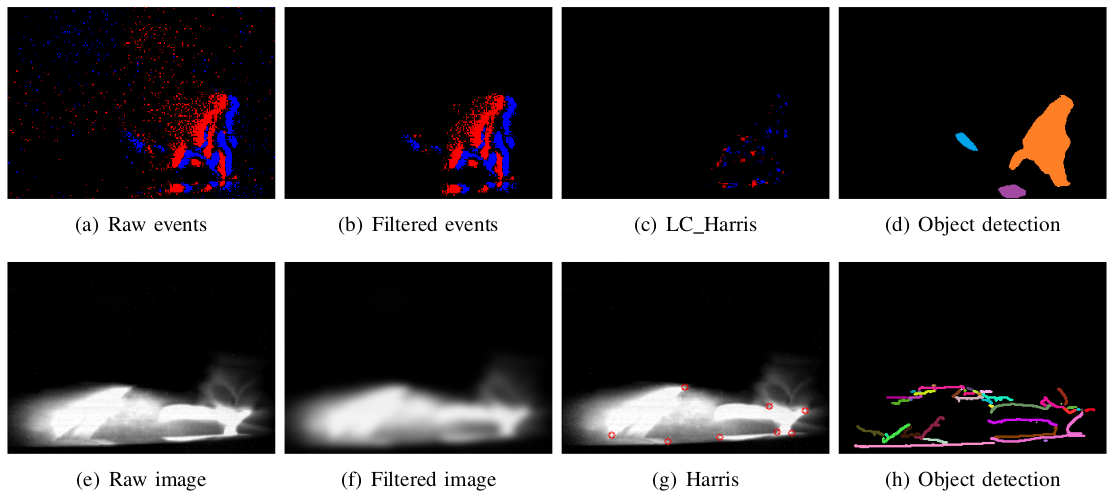
\includegraphics[width=0.8\linewidth]{images/night_obstacle.png}
    \caption{Porównanie działania algorytmu detekcji przeszkód z artykułu \cite{night_obstacle} dla DVS i~tradycyjnej kamery. Zastosowanie kamery zdarzeniowej umożliwia detekcję w nocnych warunkach.}
    \label{fig:night_obstacle}
\end{figure}

System detekcji przeszkód z projektu \cite{night_obstacle} działa w następujący sposób:
\begin{enumerate}
    \item Filtracja szumu tła -- w danych otrzymywanych z~kamery zdarzeniowej występują błędnie wygenerowane zdarzenia, które nie są częścią właściwego sygnału i~które należy z~niego usunąć w~celu obniżenia wymagań obliczeniowych dla późniejszych etapów (mniej zdarzeń do przetworzenia) oraz zwiększenia niezawodności algorytmu. W tym celu użyto algorytmu kNN (ang. \textit{k-nearest neighbour}) \cite{dba_filter}.
    \item Podział odczytywanych zdarzeń na grupy, jako które będą dalej przetwarzane. Do każdej \textit{klatki}, zapisywane jest $N$ zdarzeń. Wartość $N$ dobierana jest dynamicznie w~zależności od prędkości obiektów.
    \textit Dopasowanie płaszczyzn w~chmurze punktów -- zdarzeń, do poszczególnych obiektów na~scenie za pomocą algorytmu RHT (ang. \textit{Randomised Hough Transform}).
    \item Wyznaczenie punktów charakterystycznych za pomocą metody bazującej na algorytmie Harris \cite{Harris}. 
    \item Estymacja głębi dla każdej z przeszkód. Autorzy mimo zastosowania pojedynczej kamery, obliczają odległość za pomocą triangulacji, dzięki danym o pozycji i rotacji kamery.
\end{enumerate}

\begin{figure}
    \centering
    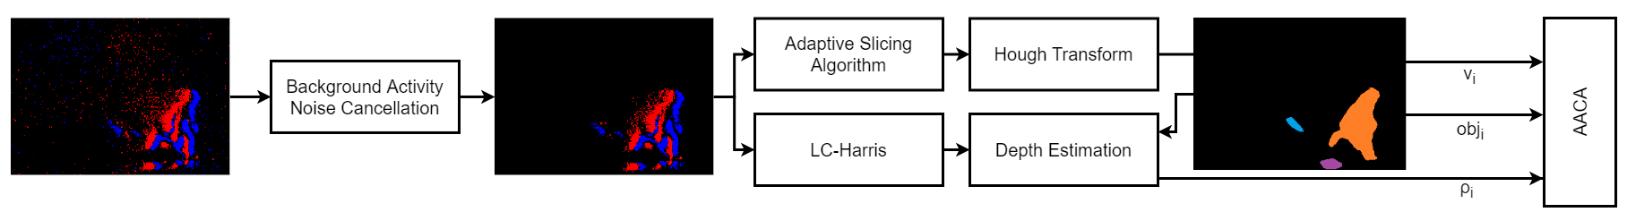
\includegraphics[width=1\linewidth]{images/overview_night_obstacle.png}
    \caption{Schemat działania algorytmu detekcji z~projektu \cite{night_obstacle}.}
    \label{fig:night_overview}
\end{figure}
    
%TODO tu by się przydało wymienić (choćby po 1 zdaniu) jeszcze kilka artykułów, może tych, które są wymienione poniżej: RED, ASTMNet itd.


% \section{Detekcja obiektów}

% Wykrywanie obiektów za pomocą danych z kamer zdarzeniowych







Innym, często spotykanym podejściem do wykrywania obiektów za pomocą kamer zdarzeniowych, jest użycie uczenia maszynowego i~głębokich sieci neuronowych. Tego typu modele do detekcji zostały stworzone w~ramach wielu dostępnych w~literaturze projektów i~stanowią bogatą bazę narzędzi. Przykładowo wymienić można algorytmy:
\begin{itemize}
    \item \textit{RED} \cite{RED} -- wprowadza rekurencyjną architekturę, umożliwiającą uczenie na podstawie zdarzeń bez konieczności rekonstrukcji obrazu,
    \item \textit{ASTMNet} \cite{ASTMNet} -- wykorzystuje moduł pamięci do detekcji obiektów w~sposób ciągły, eliminując potrzebę przekształcania zdarzeń na obrazy,
    \item \textit{RVT} \cite{RVT} -- redukuje czas przetwarzania do \SI{12}{\micro\s} przy zachowaniu wysokiej wydajności i~efektywności parametrów,
    \item \textit{DMANet} \cite{DMANet} -- wykorzystuje podwójną pamięć (modeluje ją jako krótko i długotrwałą) do skutecznej agregacji zdarzeń dla lepszej detekcji obiektów,
    \item \textit{TEDNet} \cite{TEDNet} -- wprowadza etykiety widoczności obiektów i~strategie ich śledzenia, umożliwiając detekcję w~przypadku braku relatywnego ruchu wobec kamery.
\end{itemize}

% \section{Inne wykorzystane projekty} % Może raczej wykorzystywane projekty, też: Śledzenie obiektów SORT 

% O v2e, ESim, SORT

% W literaturze można znaleźć wiele artykułów opisujących projekty, których autorzy stworzyli gotowe i~wygodne do wykorzystania w kodzie narzędzia, spełniające różne zadania, których realizacja w ramach tego projektu była wymagana. Użycie takich narzędzi ułatwia pracę oraz pozytywnie wpływa na efekt końcowy.

% \vspace{11px}
% \noindent \textbf{Symulacja DVS na podstawie klatek z tradycyjnej kamery}
% \vspace{11px}



% \vspace{11px}
% \noindent \textbf{Śledzenie obiektów}
% \vspace{11px}

% Problem śledzenia obiektów polega na przypisywaniu do nich indywidualnych identyfikatorów, tak aby możliwe było ich jednoznaczne rozpoznanie w kolejnych iteracjach algorytmu.
% W projekcie wykorzystywane jest do tego celu narzędzie SORT (ang. \textit{Simple Online and Real-time Tracking}) \cite{sort}, którego zaletą jest łatwość użycia w skryptach w języku Python.










        
        \chapter{Symulacja Software in the Loop}
\label{cha:symulacja}

% w tym rozdziale też jakieś screeny, wykresy, parametry itp.
% przebieg testów wraz z uzasadnieniem i komentarzem odnośnie wyników itp.

Pierwszym elementem, który w ramach projektu należało stworzyć, jest symulacja SiL (ang. \textit{Software in the Loop}). Celem jest otrzymanie narzędzia, które pozwoli na wygodne i~szybkie testowanie tworzonego w późniejszym etapie algorytmu detekcji przeszkód.

Przed przystąpieniem do realizacji zadania, warto zdefiniować wymagania i~oczekiwania, jakie są postawione przed gotowym oprogramowaniem:
\begin{enumerate}
    \item Symulacja powinna umożliwić testowanie dla różnych scenariuszy (np. inne przeszkody w~zmiennych pozycjach).
    \item W symulacji należy umieścić robota/drona, wyposażonego w~odpowiednie czujniki, z~których dane powinny być łatwo dostępne.
    
    Jako pojazd przenoszący kamerę zdarzeniową, dla którego będą wykrywane przeszkody, został wybrany czterowirnikowy dron. Taka decyzja uwarunkowana była kilkoma czynnikami:
    \begin{itemize}
        \item Zachowana zostaje analogia do analizowanych w~ramach przeglądu literatury projektów, w~których również wykorzystywano podobny pojazd. Ułatwia to wzorowanie się na zastosowanych w publikacjach metodach. 
        %Ułatwia to porównanie niniejszej pracy z publikacjami z literatury.
        \item Dron ma szerokie możliwości unikania wykrytych przeszkód, a~więc pełnego wykorzystania dostarczonych mu przez algorytm danych. Dzięki temu możliwości pojazdu nie będą ograniczeniem dla efektywności algorytmu sterującego, korzystającego z~informacji o~przeszkodach.
    \end{itemize}
    \item Użytkownik powinien mieć możliwość sterowania (za pomocą napisanego kodu) robotem/dronem poruszającym się po scenie symulacji.
    \item Symulacja powinna dostarczać dane z~kamery zdarzeniowej, umieszczonej na robocie/dronie.
\end{enumerate}



\section{Symulacja w Gazebo}
\label{sec:sym_gazebo}

Jako środowisko symulacyjne, w~którym całość została zrealizowana, wybrano oprogramowanie Gazebo.

% Jakbym chciał, żeby tu było więcej stron, to można jakieś loga tych narzędzi powrzucać czy jakieś scrreny przykładowe
% O Gazebo, Co to? Można potem przeniść do teorii

\textbf{Gazebo} jest otwartoźródłowym symulatorem robotyki, wykorzystywanym do testowania i~rozwijania algorytmów sterowania robotami w~realistycznym, trójwymiarowym środowisku. Zapewnia dostęp do zaawansowanego modelu fizyki oraz wielu czujników. Jest zintegrowany z~platformą programistyczną ROS2. Gazebo umożliwia umieszczanie na scenie zarówno obiektów statycznych, jak i~ruchomych. % -- taką rolę mogą pełnić na przykład chodzący szybkim krokiem ludzie.
Symulator pozwala też na stworzenie nocnej sceny.

\vspace{11px}
% Dlaczego gazebo
\noindent Oprócz wspomnianych funkcjonalności, Gazebo jest środowiskiem, które świetnie nadaje się do zastosowania w~projekcie z~dwóch głównych powodów:
\begin{itemize}
    \item Gazebo jest wspierane przez inne narzędzia, których użycie jest konieczne; w~szczególności ważna jest możliwość użycia wykorzystywanego w~projekcie narzędzia do sterowania lotem drona w~symulacji,
    \item Gazebo wykorzystuje i~wspiera użycie \textit{frameworka} ROS2, który jest konieczny do sterowania dronem oraz odczytywania danych z~czujników.
\end{itemize}

% O PX4

W celu umieszczenia w symulacji drona oraz zapewnienia możliwości sterowania nim należy wykorzystać odpowiednie oprogramowanie. Do tego celu wybrany został system \textbf{PX4 Autopilot}. Jest to zaawansowane, \textit{open-source}'owe oprogramowanie sterujące dla bezzałogowych statków latających (ale również dla innych robotów mobilnych). Jest jednym z najczęściej wykorzystywanych systemów autopilota w dziedzinie robotyki powietrznej i autonomicznych pojazdów, wspieranym przez aktywną społeczność i dużą liczbę integracji z różnorodnym sprzętem. Najważniejszymi dla projektu zaletami tego systemu są:
\begin{itemize}
    \item Wsparcie dla czterowirnikowych dronów,
    \item Możliwość sterowania za pomocą zewnętrznego oprogramowania, wykorzystując ROS2 -- tryb Offboard.
\end{itemize}

% O ROS2 - coś więcej o ROSie można potem dopisać w teorii - wyjąsnić jak działają węzły, topici i message, wtedy tu można skrócić



% Jak spełniłem kolejne wymagania z listy 
% \vspace{11px}
% \noindent \textbf{Realizacja}
% \vspace{11px}
\subsection{Przygotowanie środowiska}

Pierwszym krokiem realizacji symulacji była instalacja i przygotowanie środowiska. Dla systemu Linux w dystrybucji Ubuntu 22.04 pobrane zostały:
\begin{itemize}
    \item ROS2 w dystrybucji Humble,
    \item Symulator Gazebo,
    \item Python 3.10.
\end{itemize}

% Stworzenie świata w gazebo - konfiguracja z ROSem i PX4, wykorzytsanie gotowego przykładu - spełnienie wymagania 2 i 3

W celu umieszczenia drona w środowisku symulacyjnym i umożliwienia sterowania nim, wykorzystany został system PX4 Autopilot. Należy go odpowiednio skonfigurować do pracy z Gazebo i ROS-em, tak żeby było możliwe pisanie własnych węzłów (ang. \textit{node}) w Pythonie. Są to procesy, których zadaniem będzie na przykład sterowanie dronem lub przetwarzanie danych z czujników.

Ponieważ konfiguracja wszystkich narzędzi, tak by skutecznie ze sobą współpracowały, jest zadaniem stosunkowo trudnym -- szczególnie dla nowego użytkownika, warto skorzystać z gotowego przykładu i~dołączonej do niego instrukcji konfiguracji. Dzięki temu, dopóki dokładnie wykonuje się opisane kroki, zyskuje się względną pewność, że błędy popełnione na tym etapie nie utrudnią realizacji zadania w~przyszłości. Taki przykład dostępny jest na Githubie pod linkiem: \url{https://github.com/ARK-Electronics/ROS2_PX4_Offboard_Example}. Autorzy tego projektu poprawnie skonfigurowali go i~przygotowali do dalszej rozbudowy dla innych użytkowników.

Zawarte w przykładzie funkcjonalności obejmują:
\begin{itemize}
    \item Podstawowa, pusta scena w symulatorze Gazebo z umieszczonym w~niej czterowirnikowym dronem dostępnym w PX4 Autopilot,
    \item Przykład sterowania dronem, w~którym jako wartość zadana używany jest wektor prędkości -- na tej podstawie nowemu użytkownikowi łatwiej jest stworzyć własny system sterowania,
    \item Zaimplementowane zostało sterowanie kierunkiem i prędkością ruchu drona za pomocą strzałek na klawiaturze -- ta funkcjonalność nie jest wymagana w projekcie, jednak jest ciekawym przykładem, na podstawie którego można rozbudowywać symulację,
    \item Dodatkowy moduł wizualizacji, wykorzystujący narzędzie \textit{rviz}, służący do wyświetlenia ścieżki, jaką dron przebył w czasie trwania symulacji -- ten moduł również nie jest niezbędny, ale stanowi interesujący dodatek,
    \item Uruchamianie wszystkich modułów symulacji za pomocą jednej komendy, co znacząco ułatwia późniejsze z niej korzystanie.
\end{itemize}

Po dostosowaniu przykładu do zastosowania w projekcie, otrzymuje się gotową do dalszej pracy platformę, w której możliwe jest kontrolowanie drona za pomocą kodu pisanego w języku Python oraz obsługa danych z czujników.

Model drona wykorzystywany w symulacji to x500 (rys. \ref{fig:x500}) (nazwa używana w dokumentacji PX4). Jest on wyposażony w czujnik IMU (ang. \textit{inertial measurement unit}), który składa się z akcelerometru i żyroskopu i dostarcza danych o ruchu i orientacji drona w przestrzeni, niezbędnych do skutecznego sterowania nim.

% Screen drona

\begin{figure}
    \centering
    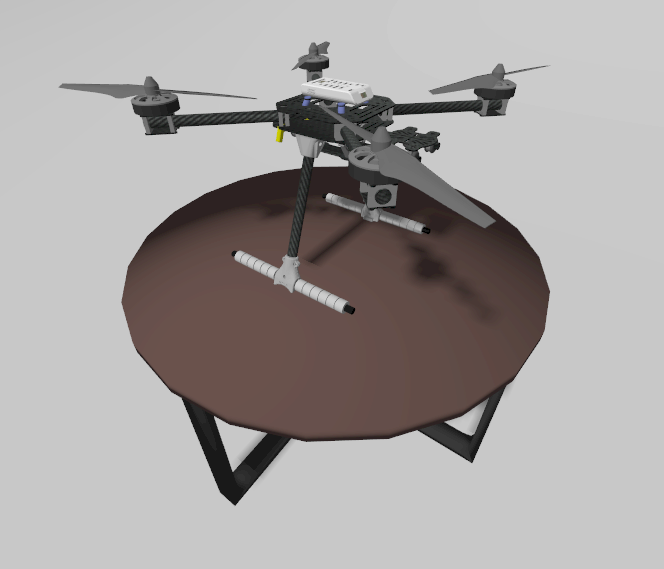
\includegraphics[width=0.5\linewidth]{images/x500.png}
    \caption{Model drona x500, dostępny w PX4 w symulacji w środowisku Gazebo.}
    \label{fig:x500}
\end{figure}

% Wymaganie 1 - losowe generowanie toru przeszkód
% \vspace{11px}
% \noindent \textbf{Losowe generowanie toru przeszkód}
% \vspace{11px}

\subsection{Losowe generowanie toru przeszkód}
\label{subsec:tor}

Dron powinien móc poruszać się w~scenie zawierającej statyczne przeszkody, które mógłby wykrywać i~omijać. 
W celu zapewnienia zmiennych warunków, w~jakich algorytm będzie testowany, należy stworzyć losowo generowany tor przeszkód. Żeby to osiągnąć, przygotowano odpowiedzialny za to skrypt w Pythonie.

Świat symulacji w~Gazebo generowany jest na podstawie kodu zawartego w~pliku \textit{.sdf}. To w~nim definiuje się używane pluginy (czyli moduły odpowiedzialne za różne zadania), czujniki, a~także umieszcza obiekty i~decyduje o~ich położeniu. Skrypt generujący przeszkody uruchamia się za każdym razem, gdy włączana jest symulacja, i~umieszcza obiekty w odpowiednim miejscu w kodzie w pliku \textit{.sdf}.

\vspace{11px}

Działanie skryptu generującego przeszkody:
\begin{itemize}
    \item Przekazanie parametrów wejściowych:
    \begin{itemize}
        \item Liczba przeszkód,
        \item Lista nazw przeszkód -- wybór z~trzech dostępnych: drzewo iglaste, drewniany słup energetyczny, szeroki cylindryczny słup,
        \item Obszar, który ma być pokryty przeszkodami,
        \item Minimalny dystans między dwoma obiektami,
    \end{itemize}
    \item Losowe wygenerowanie pozycji i~orientacji dla każdej przeszkody, tak by zachowany był minimalny dystans między nimi,
    \item Odpowiednie sformatowanie tekstu i~wpisanie go do pliku \textit{.sdf}.
\end{itemize}

Oprócz przeszkód w~symulacji umieszczony został jeszcze stolik -- stanowisko startowe dla drona, oraz bramka oznaczająca metę -- cel trasy drona.
Wszystkie wykorzystane obiekty pochodzą z~szerokiej biblioteki modeli dostępnych za darmo dla Gazebo: Gazebo Fuel. Łatwo dostępne modele dostosowane do szybkiego użycia w~symulacji to kolejna z zalet tego środowiska.

Dodatkowo można symulować ograniczone warunki oświetleniowe przez ręczne zmiany intensywności oświetlenia w~pliku \textit{.sdf}. 

Przykładowe sceny można zobaczyć na rysunku \ref{fig:sceny}.

% Może taki ładny screen z modelami przykładowych statycznych przeszkód, jak po prostu stoją obok siebie
% \begin{figure}
%     \centering
%     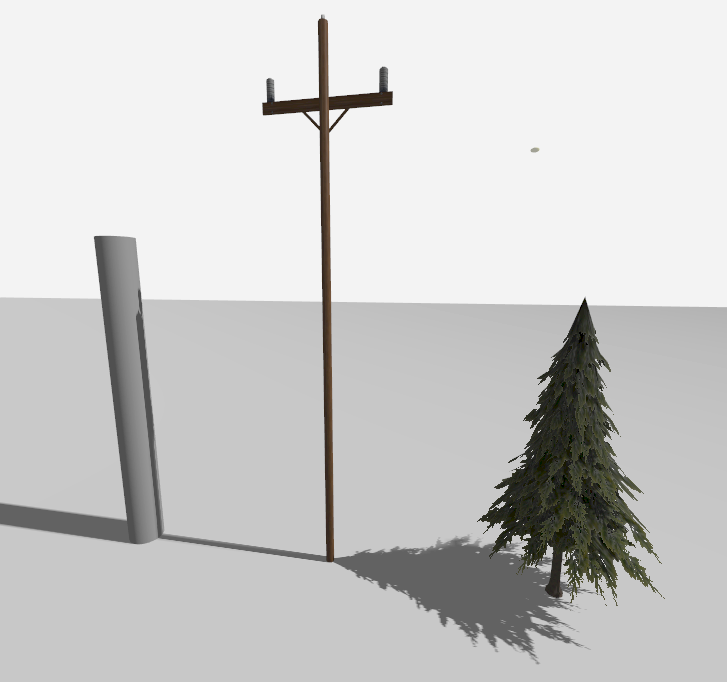
\includegraphics[width=0.5\linewidth]{images/obstacles.png}
%     \caption{Obiekty, które mogą zostać umieszczone na trasie drona, pozyskane z biblioteki Gazebo Fuel.}
%     \label{fig:obiekty}
% \end{figure}

% Ze dwa screeny sceny
\begin{figure}
    \centering
    \begin{minipage}{0.4\textwidth}
        \centering
        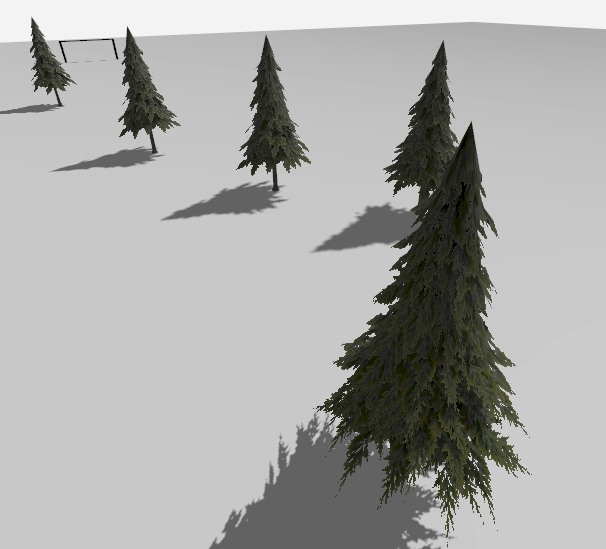
\includegraphics[width = 0.9\textwidth]{images/Track1.png}
        % \captionsetup{justification=centering}
        % \caption{}
    \end{minipage}\hfill
    \begin{minipage}{0.6\textwidth}
        \centering
        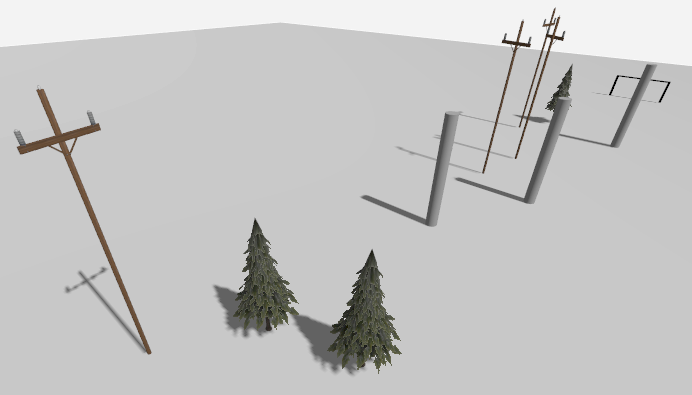
\includegraphics[width = 0.95\textwidth]{images/Track2.png}
        % \captionsetup{justification=centering}
        % \caption{}
    \end{minipage}
    \caption{Przykłady losowo wygenerowanego toru przeszkód dla drona.}
    \label{fig:sceny}
\end{figure}

% Wymaganie 4 - Symulanie DVS - próba prostego podejścia i wykorzystanie v2e
% \vspace{11px}
% \noindent \textbf{Umieszczenie w symulacji kamery zdarzeniowej}
% \vspace{11px}

\subsection{Umieszczenie w symulacji kamery zdarzeniowej}

Pomimo że w bibliotekach środowiska Gazebo dostępnych jest wiele czujników, brakuje gotowego symulatora kamery zdarzeniowej. Dla projektu, w~którym stanowi ona podstawowy element, jest to poważny problem. Jednak dzięki znajomości sposobu działania DVS, można podjąć próbę przybliżenia otrzymywanych z tego czujnika danych za pomocą zwykłej kamery.

W pierwszej kolejności należy umieścić na dronie tradycyjną kamerę. Ta jest dostępna w~Gazebo w~ramach pakietu \textit{gz-sensors}. Rozdzielczość kamery ustawiona jest na $240 \times 180$, co odpowiada rozdzielczości kamery zdarzeniowej dostępnej na rynku i powszechnie używanej (na przykład w~\cite{night_obstacle}) DAVIS240. Wykorzystując ROS-a, stworzony został węzeł, w którym dane z~kamery były na bieżąco odczytywane i~przekształcane do postaci klatek obrazu, a~następnie dalej przetwarzane.

Kamera zdarzeniowa generuje zdarzenia z~każdą zmianą jasności piksela o~stały próg. Najprostszy sposób na ich otrzymanie na podstawie klatek obrazu tradycyjnej kamery może więc wyglądać następująco:
\begin{itemize}
    \item Dwie kolejne klatki obrazu zostają od siebie odjęte (najpierw bieżąca klatka od poprzedniej, a~następnie w~odwrotnej kolejności, aby otrzymać zdarzenia o~dodatniej i~ujemnej zmianie jasności),
    \item Wynikowe obrazy są progowane przy zastosowaniu stałego progu,
    \item Z tak otrzymanych masek odczytywane są wartości położenia $x$ i $y$, dla wszystkich niezerowych pikseli i~zapisywane jako zdarzenie razem z~informacją o aktualnym czasie (ang. \textit{timestamp}) i~polaryzacji (ang. \textit{polarity}).
\end{itemize}

Takie proste podejście zostało zaimplementowane jako osobny moduł symulujący kamerę zderzeniową. Odczytuje on klatki z~kamery, a~następnie symuluje wyjście DVS, publikując przygotowane w~tym celu własne wiadomości (ang. \textit{messages}), zawierające odczytane zdarzenia.

Dodatkowo porównano wyjście symulowane tą metodą z~wyjściem rzeczywistego DVS, za pomocą zbioru danych pochodzących z~kamery zdarzeniowej DAVIS240 \textit{shapes rotation} \cite{dvs_dataset}. Przykładowe porównanie \textit{event frame}'ów jest widoczne na rysunku \ref{fig:frames_comp}. Na klatce, na której reprezentowane są zdarzenia pochodzące z~uproszczonej metody symulowania DVS, piksele (poza szarym tłem) przyjmują wyłącznie wartości skrajne (czarny, biały). Oznacza to, że nie ma różnicy w~czasie ich powstania -- wszystkie zostały wygenerowane w jednym momencie przez odjęcie dwóch klatek obrazu. Dodatkowo na klatce z~v2e widoczny jest szum.

\begin{figure}
    \centering
    \begin{minipage}{0.5\textwidth}
        \centering
        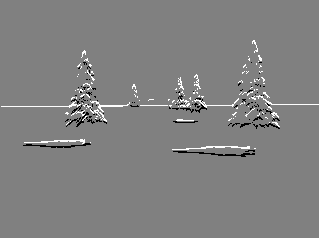
\includegraphics[width = 0.9\textwidth]{images/my_dvs_frame.png}
        \label{gra:my_dvs_frame}
    \end{minipage}\hfill
    \begin{minipage}{0.5\textwidth}
        \centering
        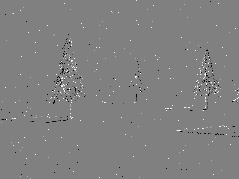
\includegraphics[width = 0.9\textwidth]{images/v2e_frame.png}
        \label{gra:v2e_frame}
    \end{minipage}
    \caption{Przykładowe \textit{event frame}'y dla uproszczonego symulatora DVS (po lewej) oraz v2e (po prawej). Słabo widoczne kształty obiektów na klatce z v2e są wynikiem ograniczonej liczby zdarzeń na jednej klatce i szumu.}
    \label{fig:frames_comp}
\end{figure}

Niestety, mimo że w korzystnych warunkach oświetleniowych i~przy niskich prędkościach względnych obiektów, \textit{event frame} wygląda bardzo podobnie do tego otrzymanego z~rzeczywistych zdarzeń, to tak mocno uproszczone podejście nie może być zastosowane w~celu symulacji DVS. Decyduje o tym kilka czynników:
\begin{itemize}
    \item Jak łatwo zauważyć, w~ten sposób traci się wszystkie z~istotnych zalet kamery zdarzeniowej -- zdarzenia rejestrowane są dokładnie wtedy kiedy klatki obrazu i~z~taką samą czułością, jaką dysponuje tradycyjna kamera,
    \item W przypadku szybciej poruszających się obiektów, liczba klatek na sekundę, jaką rejestruje kamera, może okazać się niewystarczająca -- wtedy zdarzenia pozytywne i negatywne rozdzielają się, co zmniejsza jakość otrzymywanych danych,
    \item W takim podejściu brakuje uwzględnienia szumów, jakie występują w rzeczywistej kamerze zdarzeniowej.
\end{itemize}

Oczywiście nie wszystkie z tych problemów da się całkowicie wyeliminować, ponieważ tak naprawdę czujnikiem zbierającym dane jest zwykła kamera. Można je natomiast ograniczyć przez zastosowanie bardziej dopracowanego systemu symulującego DVS.

% O v2e
\vspace{11px}

Zaawansowane i~dopracowane sposoby na konwersję klatek obrazu z~tradycyjnej kamery na zdarzenia można znaleźć w~literaturze. Kilka z~nich jest zaimplementowanych jako gotowe do użycia narzędzia. Przykładem takiego projektu może być ESIM \cite{ESIM} lub v2e \cite{v2e}.

Do zastosowania w projekcie wybrane zostało v2e, ponieważ oprócz funkcji otrzymywania zdarzeń z wcześniej nagranego filmu, oferuje ono przygotowaną do użycia w~Pythonie bibliotekę, która umożliwia konwersję kolejnych klatek obrazu na zdarzenia w~czasie rzeczywistym. Dzięki temu v2e można zastosować w~węźle ROS-a. 

\textbf{v2e} to \textit{framework} stworzony w~Pythonie, który umożliwia konwersję klatek obrazu ze zwykłej kamery na możliwie realistyczny i~odpowiadający pierwowzorowi strumień zdarzeń. Proces symulacji (na rys. \ref{fig:v2e}) jest wieloetapowy i~obejmuje:
\begin{itemize}
    \item Interpolację klatek, w celu zwiększenia ich częstotliwości, za pomocą narzędzia SuperSloMo \cite{SuperSloMo},
    \item Uwzględnienie logarytmicznej skali, w jakiej działają piksele DVS,
    \item Generację zdarzeń dla każdego piksela na podstawie zmian jasności na poszczególnych klatkach,
    \item Dodanie do sygnału szumów, występujących w rzeczywistych kamerach zdarzeniowych.
\end{itemize}

\begin{figure}
    \centering
    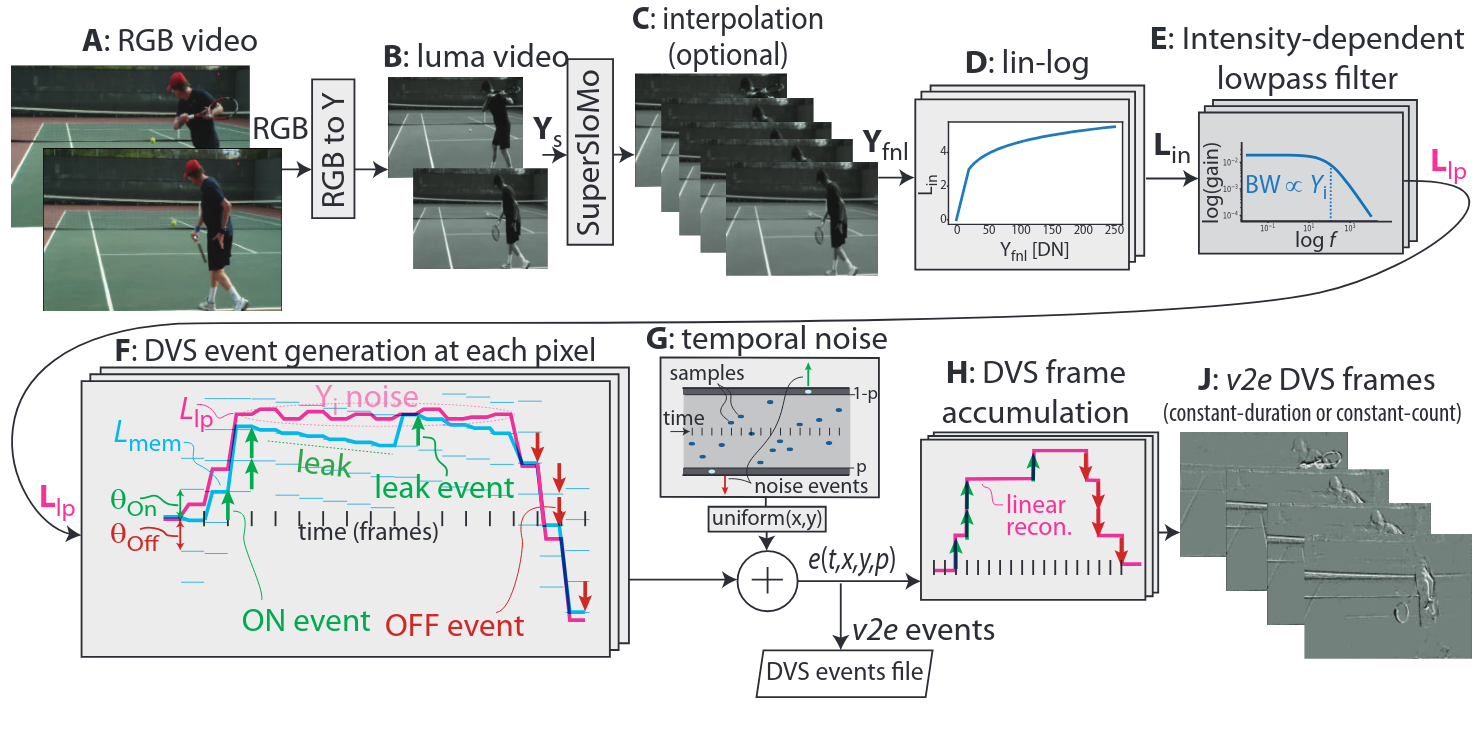
\includegraphics[width=0.85\linewidth]{images/v2e_overview.png}
    \caption{Schemat działania symulacji kamery zdarzeniowej w v2e \cite{v2e}.}
    \label{fig:v2e}
\end{figure}

% Podniesie FPS, żeby poprawić wydajność
Wspomniany emulator ma istotną wadę -- nie pozwala w pełni wykorzystać zalet systemu v2e. Ponieważ narzędzie SuperSloMo \cite{SuperSloMo}, stosowane do interpolacji klatek i~zwiększenia FPS (ang. \textit{frames per second} -- klatki na sekundę) sygnału wejściowego, wymaga zarówno obecnej, jak i~przyszłej klatki obrazu, nie jest możliwe jego zastosowanie bez wprowadzenia dodatkowej latencji.
Wobec tego sposobem na poprawę jakości danych wejściowych kamery jest podniesienie jej FPS. Im większa dynamika sceny (prędkość obiektów), tym bardziej rośnie wymagana wartość FPS. Niestety, wzrost tej wartości znacząco wpływa na wymagania obliczeniowe symulacji i~jakość jej wykonania. Wobec tego, FPS ustawiane jest na najwyższą możliwą wartość, która nie spowalnia działania symulacji zbyt mocno. Testy przeprowadzane były przy wartości $100$ -- zdecydowanie zbyt niskiej dla szybko poruszających się obiektów, jednak należało wziąć pod uwagę ograniczenia sprzętowe.

% \vspace{11px}
% \noindent Poprzednio stworzony moduł został zamieniony na nowe rozwiązanie.

% Tutaj można też napisać o wizualizacji, czyli o agregacji event frame'ów - potem warto opisać terii o DVS

\vspace{11px}

% Poszło do teorii
% Na wyjściu emulatora v2e otrzymywana jest tablica \textit{eventów}, z których każdy zapisany jest jako krotka $(ts, x, y, p)$, gdzie: $ts$, to czas wystąpienia zdarzenia, $x$ i $y$, to jego położenie, a $p$ określa polaryzację. Taka forma danych, chociaż sprawdza się w obliczeniach komputerowych, jest trudna do zrozumienia dla człowieka. Dlatego wyłącznie w celu wizualizacji (ważnej w procesie testowania), zdarzenia są zapisywane jako \textit{event frame}'y z uwzględnieniem ich \textit{timestampów} - tak jak opisane w \cite{Blachut_2023}, przy wykorzystaniu reprezentacji \textit{exponentially decaying time surface}.


\section{Rezultaty}  % Było testy, warto o jakichś też wspomnieć, może z tymi fps-ami, ale głównie to screeny i ich opisy

% Na rysunku \ref{fig:sceny} przedstawiono wyniki uzyskane w etapie opisanym w podrozdziale \ref{subsec:tor}.



% \begin{figure}
%     \centering
%     \begin{minipage}{0.4\textwidth}
%         \centering
%         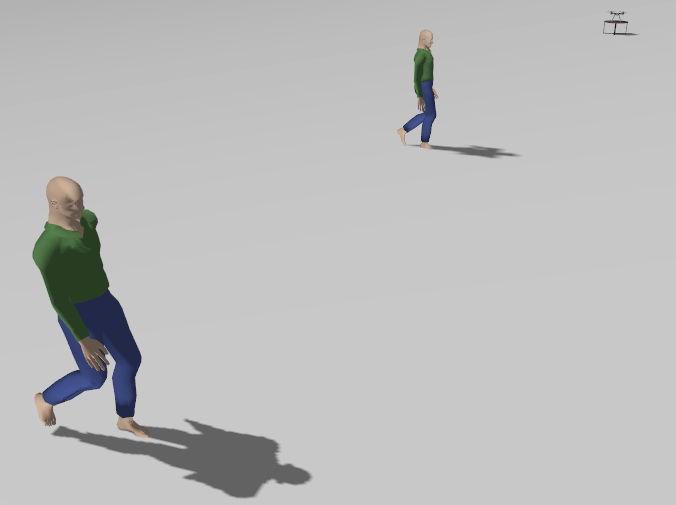
\includegraphics[width = 0.9\textwidth]{images/ludzie.png}
%     \end{minipage}\hfill
%     \begin{minipage}{0.6\textwidth}
%         \centering
%         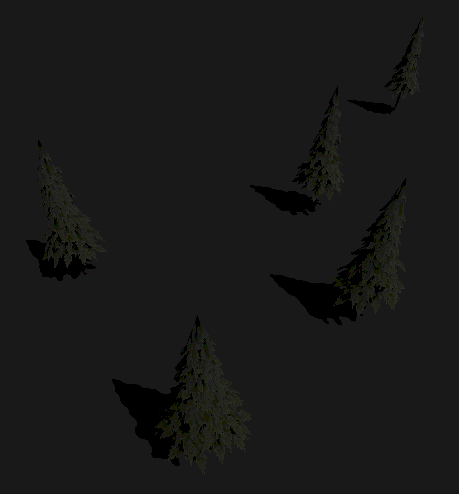
\includegraphics[width = 0.95\textwidth]{images/noc.png}
%     \end{minipage}
%     \caption{Przykłady scen możliwych do stworzenia w celu testów wykrywania przeszkód.}
%     \label{fig:sceny2}
% \end{figure}

% Screen event framów dla pierwszego i drugiego podejścia, można wrzucić błędny screen pierwszego jakby się udało uchwycić, screen widoku z kamery
% Można jeszcze wrzucić coś z testów na shapes.bag

\begin{figure}
    \centering
    \begin{minipage}{0.5\textwidth}
        \centering
        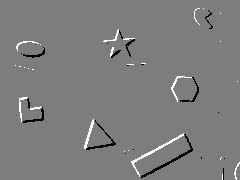
\includegraphics[width = 0.9\textwidth]{images/shapes_slow_my.png}
        \label{gra:my_dvs_shapes}
    \end{minipage}\hfill
    \begin{minipage}{0.5\textwidth}
        \centering
        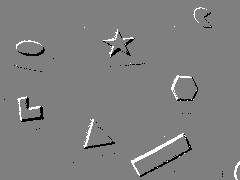
\includegraphics[width = 0.9\textwidth]{images/shapes_slow_org.png}
        \label{gra:real_shapes}
    \end{minipage}
    \caption{\textit{Event frame}'y otrzymane z~klatek obrazu za pomocą uproszczonej metody symulacji DVS (po lewej) i z~danych \textit{shapes rotation} \cite{dvs_dataset} (po prawej), dla małej prędkości ruchu kamery.}
    \label{fig:shapes_slow}
\end{figure}

\begin{figure}
    \centering
    \begin{minipage}{0.5\textwidth}
        \centering
        
\includegraphics[width = 0.9\textwidth]{images/shapes_fast_my.png}
        \label{gra:my_dvs_shapes_fast}
    \end{minipage}\hfill
    \begin{minipage}{0.5\textwidth}
        \centering
        
\includegraphics[width = 0.9\textwidth]{images/shapes_fast_org.png}
        \label{gra:real_shapes_fast}
    \end{minipage}
    \caption{\textit{Event frame}'y otrzymane z~klatek obrazu za pomocą uproszczonej metody symulacji DVS (po lewej) i z~danych \textit{shapes rotation} \cite{dvs_dataset} (po prawej), gdy kamera porusza się szybciej.}
    \label{fig:shapes_fast}
\end{figure}


Rysunki \ref{fig:shapes_slow} oraz \ref{fig:shapes_fast} zawierają porównanie uproszczonego sposobu na symulowanie DVS z \textit{event frame}'ami uzyskanymi na podstawie zbioru danych. Szczególnie obserwując \ref{fig:shapes_slow}, można ulec wrażeniu, że prosta metoda jest wystarczająco dobra i klatki niewiele się od siebie różnią. Wystarczy jednak spojrzeć na \ref{fig:shapes_fast}, żeby uświadomić sobie, że uproszczenie to jest zbyt daleko posunięte, żeby ta metoda nadawała się do zastosowania w symulacji. Przy szybkim ruchu kamery obiekty rozdzielają się, tworząc dwa osobne kształty. Generowana jest duża liczba zdarzeń. Negatywnie wpływa to zarówno na złożoność obliczeniową algorytmu detekcji, jak i jego skuteczność -- jedna przeszkoda może być wykryta jako dwie, jej rozmiar i położenie mogą nie odpowiadać rzeczywistemu.


        \chapter{Algorytm detekcji przeszkód}
\label{cha:algorytm}



        % \chapter{Implementacja na platformie wbudowanej}
\label{cha:implementacja}

tu napisać po co, jakie ograniczenia, jakie optymalizacje zostały zastosowane, jaki jest zysk - porównanie czasu wykonania, zużycia energii, zasobów względem referencyjnego modelu programowego

\section{Wykorzystywany układ}
\label{sec:plytka}



\section{Implementacja}
\label{sec:implementacja}

W jaki sposób przeniesiono system na wbudowaną platformę obliczeniową

\section{Testy HiL}
\label{sec:testy}

        \chapter{Wyniki i testy}
\label{cha:wyniki}

%TODO w miarę możliwości proszę spróbować się porównać z innymi pracami - jakaś tabelka, komentarz do wyników, ew. screeny
%+ tak jak w komentarzach poniżej - efekt filtracji, działanie śledzenia itp.

% Screeny i coś o tym dlaczego estymacja głębi nie działa
Po implementacji algorytmu w~języku Python sprawdzono jego działanie na dwa sposoby:
\begin{enumerate}
    \item Na różnych zbiorach danych z rzeczywistych kamer zdarzeniowych:
    \begin{itemize}
        \item Dla zbioru \textit{shapes rotation}, pochodzącego z~projektu \cite{dvs_dataset}. Jest to zbiór danych zarejestrowany przez przesuwanie i~obracanie kamerą zdarzeniową DAVIS240 nad powierzchnią z~umieszczonymi na niej różnorakimi kształtami. Nie są to dane zbliżone do tych, na których algorytm ma docelowo działać, lecz obecność wielu osobnych obiektów pozwala na ocenę segmentacji i~śledzenia.
        \item Dla zbioru \textit{night run}, pochodzącego z~projektu \cite{night_run}. Jest on dobrym sposobem na przetestowanie zdolności do wykrywania obiektów w~ciemności. Został stworzony przez zarejestrowanie człowieka biegnącego nocną porą przed obiektywem kamery zdarzeniowej zamocowanej na stojącym samochodzie.
    \end{itemize}
    % O ograniczeniach takiego testowania
    Testy na uprzednio zarejestrowanych zbiorach danych pozwalają na sprawdzenie działania tylko części algorytmu -- ponieważ nie ma w~nich dostępu do informacji o~parametrach zewnętrznych kamery (tj. pozycji i~orientacji), nie można przeprowadzić estymacji głębi.
    \item W~środowisku symulacyjnym Gazebo, gdzie mogą zostać przetestowane wszystkie etapy algorytmu. Testy zostały przeprowadzane dla różnych scenariuszy testowych, obejmujących:
    \begin{itemize}
        \item Sceny statyczne -- przeszkody, jakie obecne są na ścieżce drona, nie poruszają się względem otoczenia.
        \item Sceny dynamiczne -- przeszkoda to obiekt będący w ruchu.
    \end{itemize}
    W celu sprawdzenia działania algorytmu również przy ograniczonym oświetleniu, dla części sceny powtórzono test w~warunkach symulujących księżycową noc -- zachowano słabe źródło światła -- księżyc.
\end{enumerate}

\vspace{11px}
Niestety, po uruchomieniu symulacji i~odczytaniu wartości wyjściowych zauważono, że obliczane odległości drona do przeszkód nie są prawidłowe i~nie zachowują wystarczającej dokładności, żeby można było w~jakikolwiek sposób ich dalej użyć. Może być to spowodowane kilkoma czynnikami:
\begin{itemize}
    \item Metoda ta wymaga bardzo dokładnych danych o~pozycji i~rotacji kamery; dodatkowo muszą być one pobrane w~chwili wykrycia przeszkody,
    \item Błędy w~dopasowywaniu punktów charakterystycznych -- zdarzało się, że pary punktów nie były przypisane właściwie, co dodatkowo wpływało na przekłamania w~danych o~dystansie,
    \item Błędy w~procesie śledzenia obiektów -- aby metoda działała prawidłowo, wymagane są dane o~przeszkodzie z~bieżącej i~poprzedniej iteracji,
    \item Zbyt małe przemieszczenie drona między dwiema kolejnymi klatkami mogło wpłynąć na znaczne zmniejszenie dokładności -- nie sposób wyznaczyć głębię za pomocą triangulacji, jeśli dron nie przemieścił się względem przeszkody w żadnym kierunku.
\end{itemize}


Mimo wielu prób, nie udało się uzyskać poprawnych wyników, zachowując przyjętą metodę.
Brak prawidłowych danych o~dystansie do wykrytych obiektów jest poważnym problemem, który w~ostatecznej wersji algorytmu musi być rozwiązany w~inny sposób. % Potencjalne rozwiązania zaproponowano w~rozdziale \ref{sec:wnioski}.
Błąd uniemożliwia otrzymanie pozycji przeszkody w~trójwymiarowej przestrzeni, a~także powoduje niepoprawne wartości obliczanych prędkości przeszkód.

% Mimo błędnego działania ostatniej fazy algorytmu, możliwe jest przetestowanie wcześniejszych etapów i ocena jakości samej detekcji obiektów.

Algorytm realizuje zadanie detekcji obecności obiektów w~polu widzenia kamery zdarzeniowej. Dostarcza danych o~ich kształcie oraz rozmiarach i~położeniu na dwuwymiarowej płaszczyźnie obrazu. Możliwe jest przetestowanie wcześniejszych etapów i~ocena jakości samego wykrywania obiektów, pomimo błędnego działania ostatniej fazy algorytmu -- estymacji głębi.

\vspace{11px}
W pierwszej kolejności osobno sprawdzono działanie każdej z faz algorytmu.

% \vspace{11px}
% \noindent \textbf{Ocena jakości filtrowania}
% \vspace{11px}

Dzięki wizualizacji wyników filtrowania i~porównania go z oryginalnymi zdarzeniami, można ocenić jego jakość oraz dobrać parametry. Wynik działania filtru na symulacji z dodanym szumem można zobaczyć na rysunku \ref{fig:filter_example}.

% Porównanie frameów przed i po filtrowaniu - tylko jeden przykład
\begin{figure}
    \centering
    \begin{minipage}{0.5\textwidth}
        \centering
        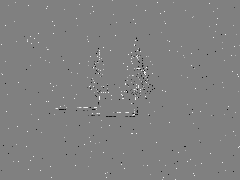
\includegraphics[width = 0.9\textwidth]{images/unfiltered_example.png}
    \end{minipage}\hfill
    \begin{minipage}{0.5\textwidth}
        \centering
        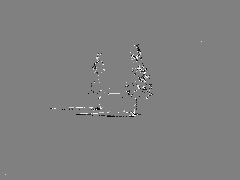
\includegraphics[width = 0.9\textwidth]{images/filtered_example.png}
    \end{minipage}
    \caption{Przykład ramki zdarzeniowej przed (po lewej) i po zastosowaniu filtracji (po prawej).}
    \label{fig:filter_example}
\end{figure}




% \vspace{11px}
% \noindent \textbf{Śledzenie przeszkód}
% może kilka kolejnych klatek z przeszkód - żeby pokazać, że są śledzone


% \vspace{11px}
% \noindent \textbf{Punkty charakterystyczne}
% Jeden screen z dopasowania cech


% \vspace{11px}
% \noindent \textbf{Testy na gotowych zbiorach danych}
% Zestawienia screenów dla zbioru danych z rzeczywistej kamery zdarzeniowej
\begin{figure}
    \centering
    \begin{minipage}{0.33\textwidth}
        \centering
        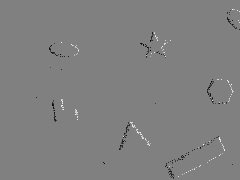
\includegraphics[width = 0.95\textwidth]{images/unfiltered_shapes1.png}
    \end{minipage}\hfill
    \begin{minipage}{0.33\textwidth}
        \centering
        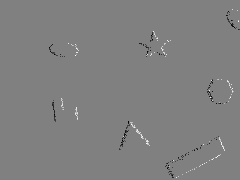
\includegraphics[width = 0.95\textwidth]{images/filtered_shapes1.png}
    \end{minipage}\hfill
    \begin{minipage}{0.33\textwidth}
        \centering
        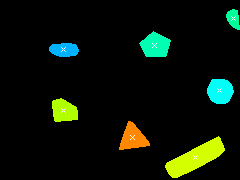
\includegraphics[width = 0.95\textwidth]{images/obst_shapes1.png}
    \end{minipage}
        \begin{minipage}{0.33\textwidth}
        \centering
        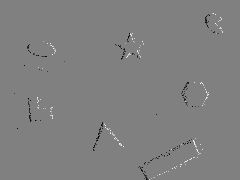
\includegraphics[width = 0.95\textwidth]{images/unfiltered_shapes2.png}
    \end{minipage}\hfill
        \begin{minipage}{0.33\textwidth}
        \centering
        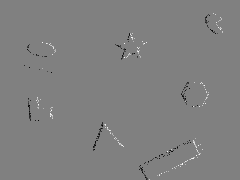
\includegraphics[width = 0.95\textwidth]{images/filtered_shapes2.png}
    \end{minipage}
    \begin{minipage}{0.33\textwidth}
        \centering
        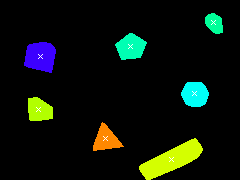
\includegraphics[width = 0.95\textwidth]{images/obst_shapes2.png}
    \end{minipage}\hfill
    \begin{minipage}{0.33\textwidth}
        \centering
        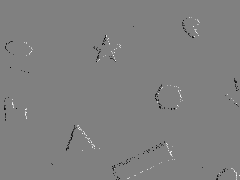
\includegraphics[width = 0.95\textwidth]{images/unfiltered_shapes3.png}
    \end{minipage}
        \begin{minipage}{0.33\textwidth}
        \centering
        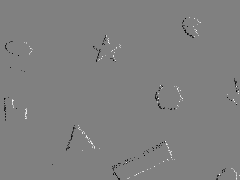
\includegraphics[width = 0.95\textwidth]{images/filtered_shapes3.png}
    \end{minipage}\hfill
    \begin{minipage}{0.33\textwidth}
        \centering
        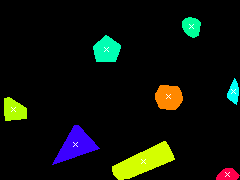
\includegraphics[width = 0.95\textwidth]{images/obst_shapes3.png}
    \end{minipage}\hfill
    \caption{Zestawienie wyników testowania algorytmu na zbiorze danych \textit{shapes rotation} w kilku wybranych momentach. Od lewej strony kolejne obrazki przedstawiają: dane przed filtracją, dane po filtracji, wykryte obiekty.}
    \label{fig:shapes_overview}
\end{figure}

\vspace{11px}

Jak można zauważyć na rysunku \ref{fig:shapes_overview}, zbiór danych \textit{shapes rotation} charakteryzuje się niewielkim szumem.
W śledzeniu obiektów czasem pojawiają się błędy -- szczególnie w przypadku zmiany kierunku ruchu obiektu. Jest to widoczne przez zmianę jego koloru. Obiekt również przestaje być śledzony, gdy znajdzie się poza polem widzenia, a następnie w nie powróci (SORT nie został wyposażony w funkcjonalność obsługującą takie przypadki). Nie jest to jednak duży problem -- algorytm wymaga jedynie możliwości porównania pozycji przeszkody z aktualnej i poprzedniej iteracji.

\vspace{11px}

Na podstawie rysunku \ref{fig:run_overview} można stwierdzić, że w~danych \textit{night run} występuje stosunkowo dużo szumu -- aby go wyeliminować, ustawiono bardziej rygorystyczne wartości parametrów filtra:
$$n=3; ~~t=\frac{1}{400}s; ~~k=6$$

W prostszym przypadku (tylko jeden poruszający się w jednym kierunku obiekt) nie występują żadne błędy w~śledzeniu -- przez cały test obiekt zachował ten sam kolor.


\begin{figure}
    \centering
    \begin{minipage}{0.33\textwidth}
        \centering
        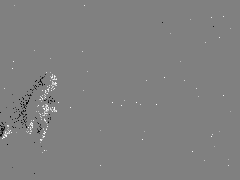
\includegraphics[width = 0.95\textwidth]{images/unfiltered_run1.png}
    \end{minipage}\hfill
    \begin{minipage}{0.33\textwidth}
        \centering
        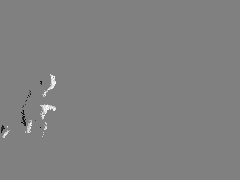
\includegraphics[width = 0.95\textwidth]{images/filtered_run1.png}
    \end{minipage}\hfill
    \begin{minipage}{0.33\textwidth}
        \centering
        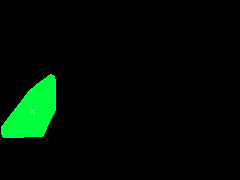
\includegraphics[width = 0.95\textwidth]{images/obst_run1.png}
    \end{minipage}
        \begin{minipage}{0.33\textwidth}
        \centering
        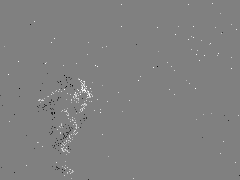
\includegraphics[width = 0.95\textwidth]{images/unfiltered_run2.png}
    \end{minipage}\hfill
    \begin{minipage}{0.33\textwidth}
        \centering
        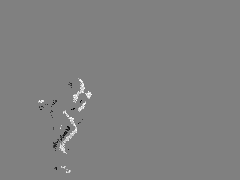
\includegraphics[width = 0.95\textwidth]{images/filtered_run2.png}
    \end{minipage}\hfill
    \begin{minipage}{0.33\textwidth}
        \centering
        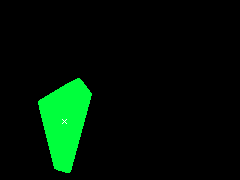
\includegraphics[width = 0.95\textwidth]{images/obst_run2.png}
    \end{minipage}
        \begin{minipage}{0.33\textwidth}
        \centering
        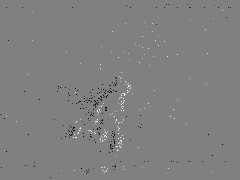
\includegraphics[width = 0.95\textwidth]{images/unfiltered_run3.png}
    \end{minipage}\hfill
    \begin{minipage}{0.33\textwidth}
        \centering
        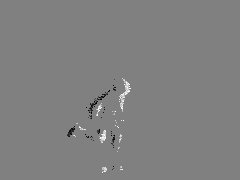
\includegraphics[width = 0.95\textwidth]{images/filtered_run3.png}
    \end{minipage}\hfill
    \begin{minipage}{0.33\textwidth}
        \centering
        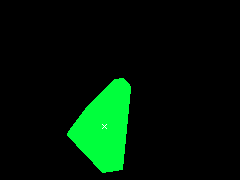
\includegraphics[width = 0.95\textwidth]{images/obst_run3.png}
    \end{minipage}
    \caption{Zestawienie wyników testowania algorytmu na zbiorze danych \textit{night run} w~kilku wybranych momentach. Od lewej strony kolejne obrazki przedstawiają: dane przed filtracją, dane po filtracji, wykryte obiekty.}
    \label{fig:run_overview}
\end{figure}


% \vspace{11px}
% \noindent \textbf{Scenariusze testowe w Gazebo}
% \vspace{11px}

\begin{figure}
    \centering
    \begin{minipage}{1\textwidth}
        \centering
        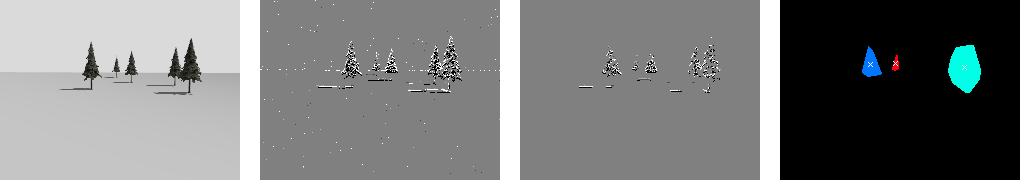
\includegraphics[width = 1\textwidth]{images/trees_day1.png}
    \end{minipage}
    \begin{minipage}{1\textwidth}
        \centering
        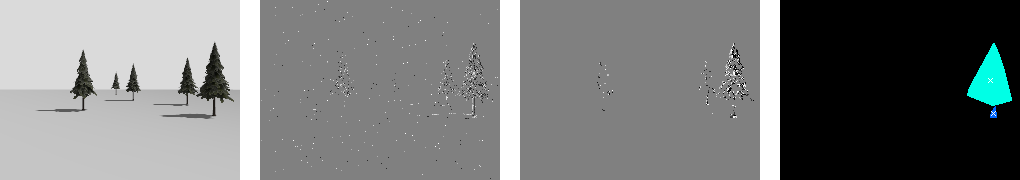
\includegraphics[width = 1\textwidth]{images/trees_day3.png}
    \end{minipage}
    \begin{minipage}{1\textwidth}
        \centering
        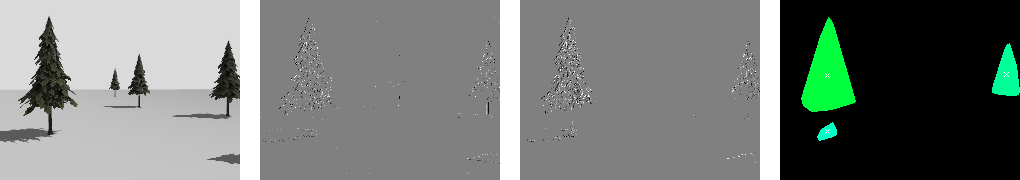
\includegraphics[width = 1\textwidth]{images/trees_day5.png}
    \end{minipage}
    \begin{minipage}{1\textwidth}
        \centering
        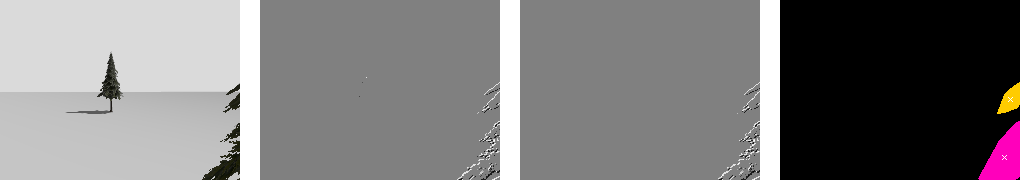
\includegraphics[width = 1\textwidth]{images/trees_day6.png}
    \end{minipage}
    \caption{Pierwszy scenariusz testowy -- statyczna scena w~dziennym świetle. Rolę przeszkód pełnią drzewa umieszczone przed lecącym naprzód dronem. Kolejne obrazki od lewej zawierają: obraz z~tradycyjnej kamery, nieprzefiltrowane dane z~DVS, dane z~DVS po filtracji, wykryte przeszkody.}
    \label{fig:trees_day}
\end{figure}

\vspace{11px}

 Na podstawie przebiegu testu sprawdzającego działanie systemu dla statycznej sceny w warunkach dziennych (rys. \ref{fig:trees_day}) można zauważyć kilka istotnych cech algorytmu:
 \begin{itemize}
     \item Algorytm często pomija przeszkody znajdujące się dalej i mające mniejszą prędkość względem drona -- jest to spowodowane głównie tym, że dane przetwarzane są w pakietach po $N$ zdarzeń. Jeśli w polu widzenia znajduje się przeszkoda, która generuje większość z nich, to zdarzenia związane z pozostałymi przeszkodami stanowią bardzo niewielką część całości, co powoduje, że są uznawane za szum -- jeśli nie na etapie filtracji, to podczas klasteryzacji. Nie jest to w jednoznaczny sposób wada -- pomijane w ten sposób przeszkody znajdują się daleko od drona i/lub poruszają się względem niego wolno. Algorytm nadaje priorytet tym, które stanowią większe zagrożenie.
     \item W przypadku gdy przeszkodami są drzewa, ich pień bywa uznawany za osobny obiekt. Podział jednej przeszkody na kilka osobnych obiektów prowadzi do niepotrzebnego wzrostu kosztu obliczeniowego.
     \item Obiekty, które w rzeczywistości znajdują się daleko od siebie, ale w klatce obrazu są blisko, uznawane są za jedną przeszkodę -- może to być jeden z czynników utrudniających triangulację.
 \end{itemize}

\begin{figure}
    \centering
    \begin{minipage}{1\textwidth}
        \centering
        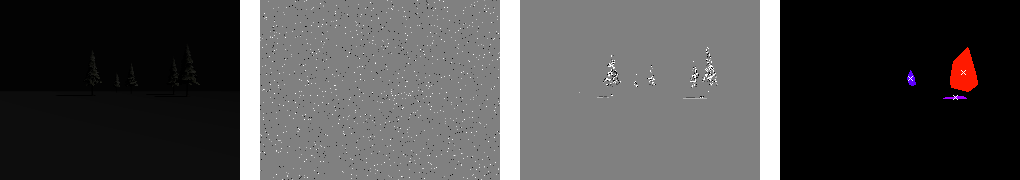
\includegraphics[width = 1\textwidth]{images/trees_night1.png}
    \end{minipage}
    \begin{minipage}{1\textwidth}
        \centering
        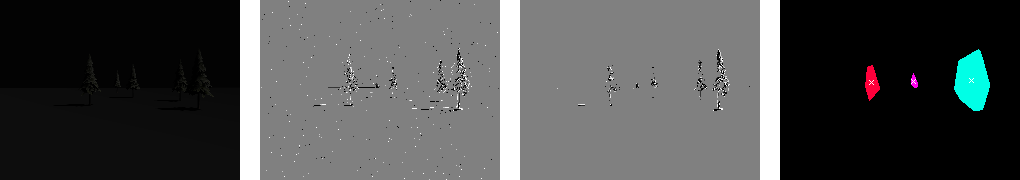
\includegraphics[width = 1\textwidth]{images/trees_night2.png}
    \end{minipage}
    \begin{minipage}{1\textwidth}
        \centering
        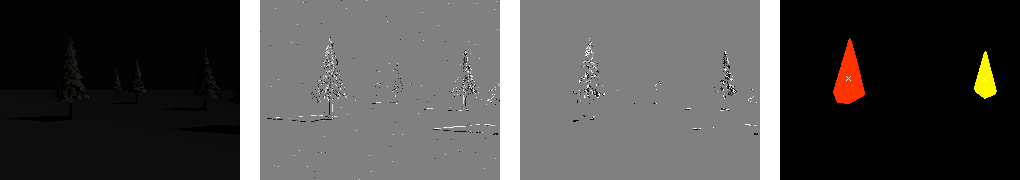
\includegraphics[width = 1\textwidth]{images/trees_night4.png}
    \end{minipage}
    \begin{minipage}{1\textwidth}
        \centering
        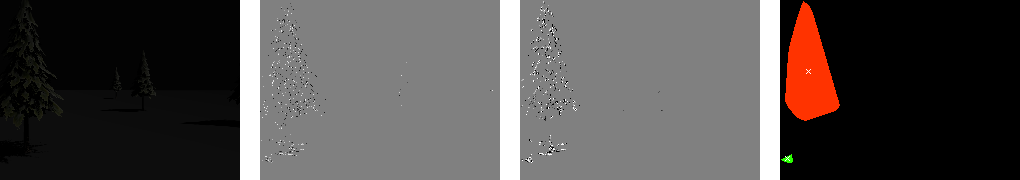
\includegraphics[width = 1\textwidth]{images/trees_night5.png}
    \end{minipage}
  
    \caption{Drugi scenariusz testowy -- statyczna scena w~nocy. Rolę przeszkód pełnią drzewa umieszczone przed lecącym naprzód dronem. Kolejne obrazki od lewej zawierają: obraz z~tradycyjnej kamery, nieprzefiltrowane dane z~ DVS, dane z~DVS po filtracji, wykryte przeszkody.}
    \label{fig:trees_night}
\end{figure}


Drugi scenariusz testowy (rys. \ref{fig:trees_night}) pokazuje, że nawet w ciemności algorytm zachowuje swoją funkcjonalność. Względem działania za dnia występują jednak pewne problemy:
\begin{itemize}
    \item Zdarza się, że jako przeszkoda rozpoznawana jest jedynie część rzeczywistego obiektu,
    \item Zaburzenia pracy algorytmu, takie jak utrata śledzonego obiektu i przypisanie do niego innego ID czy wykrycie cienia obiektu jako przeszkody, pojawiają się częściej.
\end{itemize}

\begin{figure}
    \centering
    \begin{minipage}{1\textwidth}
        \centering
        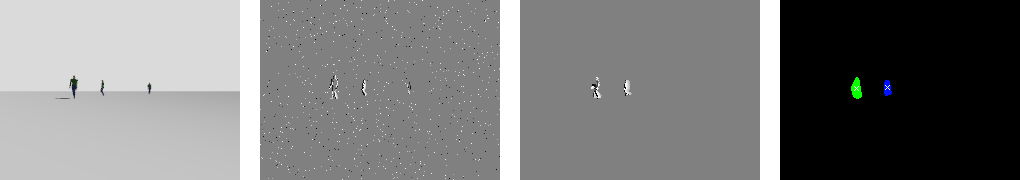
\includegraphics[width = 1\textwidth]{images/walk_day1.png}
    \end{minipage}
    \begin{minipage}{1\textwidth}
        \centering
        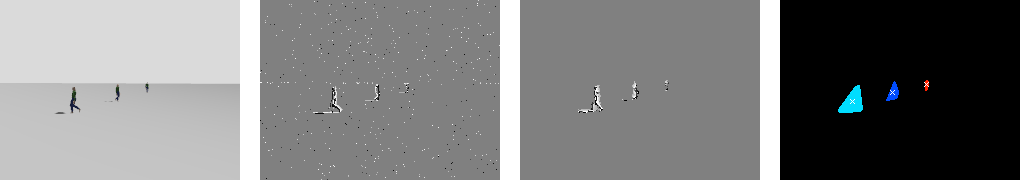
\includegraphics[width = 1\textwidth]{images/walk_day2.png}
    \end{minipage}
    \begin{minipage}{1\textwidth}
        \centering
        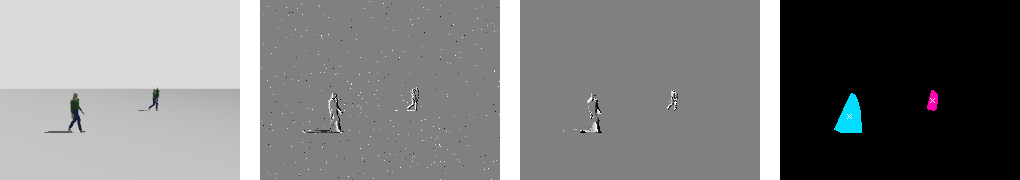
\includegraphics[width = 1\textwidth]{images/walk_day3.png}
    \end{minipage}
    \begin{minipage}{1\textwidth}
        \centering
        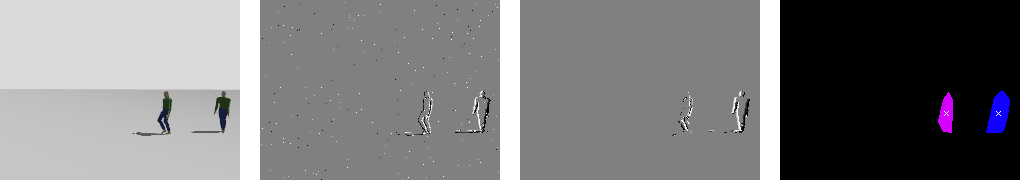
\includegraphics[width = 1\textwidth]{images/walk_day4.png}
    \end{minipage}
  
    \caption{Trzeci scenariusz testowy -- dynamiczna scena w dzień. Rolę przeszkód pełnią poruszające się szybkim krokiem ($1-1,5$ $m/s$) osoby. Kolejne obrazki od lewej zawierają: obraz z~tradycyjnej kamery, nieprzefiltrowane dane z~DVS, dane z~DVS po filtracji, wykryte przeszkody.}
    \label{fig:walk_day}
\end{figure}

\vspace{11px}

Na podstawie trzeciego testu (rys. \ref{fig:walk_day}) można stwierdzić, że poruszające się obiekty są wykrywane nawet skuteczniej niż te statyczne -- widoczne są z dalszej odległości.
Przyczyną tego jest większa liczba generowanych zdarzeń. Problemem, jaki można zaobserwować w~działaniu algorytmu, jest utrata ciągłości w śledzeniu przeszkód, gdy ludzie zmieniają kierunek ruchu lub wychodzą poza pole widzenia kamery.

\begin{figure}
    \centering
    \begin{minipage}{1\textwidth}
        \centering
        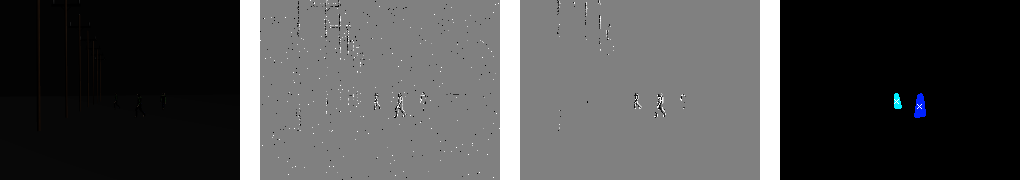
\includegraphics[width = 1\textwidth]{images/walk_night1.png}
    \end{minipage}
    \begin{minipage}{1\textwidth}
        \centering
        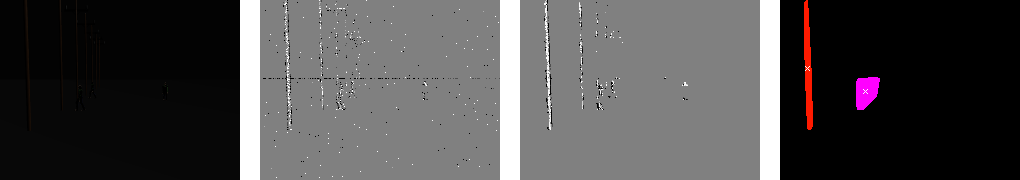
\includegraphics[width = 1\textwidth]{images/walk_night2.png}
    \end{minipage}
    \begin{minipage}{1\textwidth}
        \centering
        \includegraphics[width = 1\textwidth]{images/walk_night5.png}
    \end{minipage}
    \begin{minipage}{1\textwidth}
        \centering
        \includegraphics[width = 1\textwidth]{images/walk_night6.png}
    \end{minipage}
    \begin{minipage}{1\textwidth}
        \centering
        \includegraphics[width = 1\textwidth]{images/walk_night7.png}
    \end{minipage}
   
    \caption{Czwarty scenariusz testowy -- dynamiczna scena w nocy. Żeby utrudnić zadanie oprócz spacerujących ludzi, do sceny dodano rząd słupów energetycznych. Względem drugiego scenariusza (rys. \ref{fig:trees_night}), światła jest jeszcze mniej. Kolejne obrazki od lewej zawierają: obraz z tradycyjnej kamery, nieprzefiltrowane dane z DVS, dane z DVS po filtracji, wykryte przeszkody.}
    \label{fig:walk_night}
\end{figure}

\vspace{11px}
Z ostatnim, najtrudniejszym zadaniem (rys. \ref{fig:walk_night}), algorytm nie poradził sobie w pełni zadowalająco. W części klatek przeszkody nie były wykrywane lub były wykrywane tylko częściowo. Śledzenie obiektów stosunkowo często zawodziło -- co w znacznym stopniu utrudniałoby estymację głębi.

%Opis zalet i wad uzyskanego algorytmu
Na podstawie przeprowadzonych testów algorytmu można sformułować jego cechy -- zalety i~wady:
\begin{itemize}
    \item Gdy w~polu widzenia kamery znajduje się kilka obiektów, pośród których występują takie, które przez swoją większą prędkość lub bliższy dystans odpowiadają za generowanie wyższej liczby zdarzeń, pozostałe przeszkody nie są wykrywane. Zazwyczaj pomijane w~wyniku tego obiekty stanowią mniejsze zagrożenie dla drona, ponieważ poruszają się one wolno i/lub znajdują się daleko, więc takie zachowanie można potraktować jako zaletę -- ograniczana jest liczba wykrywanych obiektów, a~razem z~nią czas obliczeń.
    \item Algorytm dobrze radzi sobie w~ograniczonych warunkach oświetleniowych. Jak można zaobserwować na rysunkach \ref{fig:trees_night} oraz \ref{fig:walk_night}, w~pierwszej kolumnie obrazków widok z~tradycyjnej kamery jest całkowicie lub niemal całkowicie nieczytelny. Mimo to detekcja przeszkód ciągle jest możliwa, choć jej jakość nieco się zmniejsza.
    \item Typowe dla działania algorytmu błędy, których częstotliwość występowania nasila się w~bardzo trudnych warunkach oświetleniowych, to:
    \begin{itemize}
        \item Niewykrywanie obiektu na pojedynczych klatkach obrazu, co zaburza ciągłość jego działania i~powoduje dalsze błędy w śledzeniu przeszkód,
        \item Niewykrywanie całej przeszkody, a~tylko jej części -- problem dotyczy obiektów statycznych przy ograniczonym oświetleniu,
        \item Wykrywanie jednego obiektu jako kilka mniejszych przeszkód, co utrudnia śledzenie oraz może niepotrzebnie podwyższać czas potrzebny na przetwarzanie klatki.
    \end{itemize}
\end{itemize}
 


%---------------------------------%


        
    \chapter{Podsumowanie}
\label{cha:podsumowanie}

% \section{Efekty pracy i uzyskane wyniki}
% \label{sec:wyniki}

%Podsumowanie - krótko co zostało zrobione
W ramach pracy nad projektem wykonane zostały:
\begin{itemize}
    \item Przegląd literatury -- zapoznano się z metodami detekcji i~unikania przeszkód przy wykorzystaniu kamer zdarzeniowych. Przeanalizowano algorytmy wykrywania obiektów w~wybranych artykułach i~na tej podstawie stworzono własne podejście do problemu. Przeanalizowano publikacje pomocne w~jego realizacji.
    \item Środowisko symulacyjne do testów SiL -- stworzono różne scenariusze testowe (sceny), umożliwiające sprawdzenie działania algorytmu w~dziennych lub nocnych warunkach na zróżnicowanych torach przeszkód. W środowisku umieszczono model drona, wyposażonego w~kamerę zdarzeniową i~rozwiązano problem sterowania nim.
    \item Algorytm detekcji przeszkód -- zaprojektowany dzięki analizie literatury sposób działania algorytmu zaimplementowano w~języku programowania Python. Przeprowadzono wstępne próby jego działania na zbiorach danych pochodzących z~kamery zdarzeniowej DAVIS240. Używając \textit{frameworka} ROS2, przetestowano algorytm w~symulacji.
\end{itemize}

%Czego nie udało się zrobić

\vspace{11px}
Niestety, nie wszystkie cele wymienione w~rozdziale \ref{sec:celePracy} zostały osiągnięte. Z~powodu ograniczonego czasu oraz rozbudowanej formy projektu, nie udało się podjąć próby implementacji i~przetestowania rozwiązania w~formule \textit{Hardware in the Loop} na platformie wbudowanej.

% \section{Wnioski}
% \label{sec:wnioski}

%Opis zalet i wad uzyskanego algorytmu
Na podstawie testów systemu, przedstawionych i~opisanych w~rozdziale \ref{sec:algorytm_wyniki}, można zdefiniować jego cechy:
\begin{itemize}
    \item Algorytm dobrze radzi sobie w~ograniczonych warunkach oświetleniowych,
    \item Błędy w działaniu algorytmu występują częściej w ograniczonych warunkach oświetleniowych. Zazwyczaj są to:
    \begin{itemize}
        \item Niewykrywanie obiektu na pojedynczych klatkach obrazu,
        \item Wykrywanie tylko części przeszkody,
        \item Wykrywanie jednego obiektu jako kilka mniejszych przeszkód.
    \end{itemize}
\end{itemize}

Dzięki testom \textit{Software in the Loop}, możliwe było wykrycie wielu błędów i~ich naprawa na wczesnym etapie pracy nad systemem detekcji obiektów -- podczas implementacji modelu programowego.

% Czemu to co nie działa nie działa i jak by to można zrobić lepiej
W czasie testów SiL stwierdzony został poważny problem z~wartościami odległości do wykrytych obiektów zwracanymi przez algorytm. Niestety okazały się one na tyle niedokładne i~zawierały tyle błędów, że ich użycie do wyznaczania pozycji obiektów w~przestrzeni 3D oraz ich prędkości okazało się niemożliwe. Mimo podjętych prób naprawy, zachowując przyjęte podejście (triangulacja z~użyciem jednej kamery zdarzeniowej), nie udało się tego problemu rozwiązać.

Możliwe przyczyny błędnego działania tej fazy algorytmu:
\begin{itemize}
    \item Niedokładne dane o~pozycji i~rotacji kamery,
    \item Błędy w~dopasowywaniu punktów charakterystycznych,
    \item Błędy w~procesie śledzenia obiektów,
    \item Zbyt małe przemieszczenie drona między dwiema kolejnymi klatkami.
\end{itemize}

Ponieważ zastosowanie triangulacji w przypadku pojedynczej kamery okazało się błędnym podejściem, w~celu realizacji zadania rozpoznawania głębi, konieczna może okazać się zmiana metody. Proponowane rozwiązania:
\begin{itemize}
    \item Ograniczenie wykrywania do obiektów o~znanym rozmiarze -- znacznie zmniejszy to potencjalne zastosowania systemu, ale pozwoli na otrzymywanie danych o~głębi bez wyposażania drona w~dodatkowe czujniki.
    \item Umieszczenie na dronie LiDAR-u, jako dodatkowego czujnika. W tym rozwiązaniu kamera zdarzeniowa pozwoli na skuteczniejsze wykrywanie obiektów, które szybko się poruszają oraz poprawi działanie w ciemności, a~LiDAR umożliwi zwiększenie dokładności oraz pozwoli na precyzyjne odczytywanie głębi. Minusem takiego rozwiązania jest wzrost ceny oraz stopnia skomplikowania systemu. Znacznie zwiększyłaby się złożoność obliczeniowa z~powodu dodatkowych danych do przetworzenia.
    \item Zastosowanie dwóch kamer zdarzeniowych w~układzie stereo, dzięki czemu możliwe będzie przeprowadzenie triangulacji w poprawny i dokładny sposób.  % Dodatkowa masa drugiej kamery jako wada?
    \item Wybór i zastosowanie w projekcie algorytmu estymacji głębi dedykowanego dla pojedynczych kamer zdarzeniowych. Takie rozwiązania można znaleźć w literaturze na przykład w artykułach \cite{EMVS} lub \cite{single_depth}. W porównaniu do prostej koncepcyjnie triangulacji, są to rozbudowane i bardziej złożone obliczeniowo systemy.
\end{itemize}

% \section{Plany rozwoju}
% \label{sec:plany}

% plany rozwoju na przyszłość, potencjalne aplikacje, w których można zastosować algorytm itp.

\noindent Projekt ma szerokie możliwości dalszego rozwoju i~rozbudowy.

W ramach dalszej pracy nad projektem planowane jest:
\begin{itemize}
    \item Rozwiązanie problemu otrzymywania poprawnych danych o~głębi,
    \item Optymalizacja akumlacji zdarzeń do dalszego przetwarzania. Dwa podejścia do tego zagadnienia - zbieranie danych w pewnym przedziale czasowym oraz akumulacja pewnej ich liczby, można połączyć w jedno. Ten sposób pozwala na połączenie ich zalet i minimalizacje ich wad (odpowiednio możliwości wystąpienia rozmycia ruchu oraz za dużej do realizacji w czasie rzeczywistym częstotliwości ramek zdarzeniowych).
    \item Zaimplementowanie algorytmu na wbudowanej platformie obliczeniowej -- eGPU Jetson i~przetestowanie jego działania metodą HiL,
    \item Zaimplementowanie algorytmu na platformie z układem FPGA (ang. \textit{Field Programmable Gate Array}). Przeprowadzenie testów i~porównanie działania systemu uruchamianego na FPGA i~eGPU Jetson. FPGA jest platformą, która może okazać się najskuteczniejsza dla stworzonego algorytmu ze względu na szerokie możliwości zrównoleglania wykonywanych obliczeń, co w~przypadku systemów wizyjnych jest wyjątkowo efektywne.
    \item Zaprojektowanie i~implementacja systemu sterowania dronem, tak by na podstawie danych otrzymywanych z~procesu detekcji, umożliwić unikanie przeszkód,
    \item Zamontowanie systemu na rzeczywistym dronie i~przetestowanie go na przygotowanym torze przeszkód.
\end{itemize}

Mimo że algorytm detekcji testowany był z~wykorzystaniem czterowirnikowego drona, to może być zastosowany do wykrywania poruszających się względem kamery obiektów na innych rodzajach pojazdów i~wszelkich robotach mobilnych.

    
    % itd.
    % \appendix
    % \include{dodatekA}
    % \include{dodatekB}
    % itd.
    \printbibliography

    Kod projektu oraz inne pliki są dostępne w~repozytorium: 
    
    \url{https://github.com/romannowak9/DVS_Detekcja_przeszkod_Roman_Nowak}

\end{document}
